\documentclass[10pt, aspectratio=169]{beamer}
\usefonttheme{professionalfonts}
%\usetheme{CambridgeUS}
%
% Choose how your presentation looks.
%
% For more themes, color themes and font themes, see:
% http://deic.uab.es/~iblanes/beamer_gallery/index_by_theme.html
%
\mode<presentation>
{
  \usetheme{default}      % or try Darmstadt, Madrid, Warsaw, ...
  \usecolortheme{beaver} % or try albatross, beaver, crane, ...
  \usefonttheme{default}  % or try serif, structurebold, ...
  \setbeamertemplate{navigation symbols}{}
  \setbeamertemplate{caption}[numbered]
} 

\usepackage[english]{babel}
\usepackage[utf8x]{inputenc}
\usepackage{tikz}
\usepackage{pgfplots}
\usepackage{array}  % for table column M
\usepackage{makecell} % to break line within a cell
\usepackage{verbatim}
\usepackage{graphicx}
\usepackage{epstopdf}
\usepackage{amsfonts}
\usepackage{xcolor}
\usepackage{ifthen}
%\usepackage{mathtools}
\usepackage[makeroom]{cancel}
\usetikzlibrary{spy}
%\captionsetup{compatibility=false}
%\usepackage{dsfont}
\usepackage[absolute,overlay]{textpos}
\usetikzlibrary{calc, angles,quotes}
\usetikzlibrary{pgfplots.fillbetween, backgrounds}
\usetikzlibrary{positioning}
\usetikzlibrary{arrows}
\usetikzlibrary{pgfplots.groupplots}
\usetikzlibrary{arrows.meta}
\usetikzlibrary{plotmarks}
\usetikzlibrary{decorations.markings}
\usepgfplotslibrary{groupplots}
\pgfplotsset{compat=newest} 
%\pgfplotsset{plot coordinates/math parser=false}

\usepackage{hyperref}
\hypersetup{
    colorlinks=true,
    linkcolor=blue,
    filecolor=magenta,      
    urlcolor=cyan,
}

%
%\def\EXTERNALIZE{1}
%%% Page numbering
\usepackage{etoolbox} % necessary for excluding beamer-only frames from page numbering

\makeatletter
\pretocmd{\beamer@@@@frame}{\alt<#1>{}{\beamer@noframenumberingtrue}}{}{}
\makeatother

\addtobeamertemplate{navigation symbols}{}{%
	\usebeamerfont{footline}%
	\usebeamercolor[fg]{footline}%
	\hspace{1em}%
	\insertframenumber/\inserttotalframenumber
}
%%%

\definecolor{matlabcomment}{RGB}{34,139,34}

\pgfmathdeclarefunction{gauss}{1}{%
	\pgfmathparse{1/(sqrt(2*pi))*exp(-((#1)^2)/2)}%
}

\pgfmathdeclarefunction{laplacian}{2}{%
	\pgfmathparse{1/(#2*2)*exp(-(abs(x-#1))/(#2))}%
}

\pgfmathdeclarefunction{pretty_func}{1}{%
	\pgfmathparse{cos(deg(#1/2)) - sin(deg(#1)) + cos(deg(#1/2)-45) - sin(deg(#1/4)-154)}%
}

\pgfplotsset{
	dirac/.style={
		mark=triangle*,
		mark options={scale=2},
		ycomb,
		scatter,
		visualization depends on={y/abs(y)-1 \as \sign},
		scatter/@pre marker code/.code={\scope[rotate=90*\sign,yshift=-2pt]}
	}
}

\def\thickness{very thick}

\tikzset{
amark/.style 2 args={
	decoration={             
		markings, 
		mark=at position {0.5} with { 
			\arrow{stealth},
			\node[#2] {#1};
		}
	}, \thickness,
	postaction={decorate}
},
earlymark/.style 2 args={
	decoration={             
		markings, 
		mark=at position {0.25} with { 
			\arrow{stealth},
			\node[#2] {#1};
		}
	}, \thickness,
	postaction={decorate}
},
latemark/.style 2 args={
	decoration={             
		markings, 
		mark=at position {0.8} with { 
			\arrow{stealth},
			\node[#2] {#1};
		}
	}, \thickness,
	postaction={decorate}
},
zpath/.style={
	decoration={             
		markings, 
		mark=at position {0.5} with { 
			\arrow{stealth},
			\node[#1] {$z^{-1}$};
		}
	}, \thickness,
	postaction={decorate}
},
terminal/.style 2 args={draw,circle,inner sep=2pt,label={#1:#2}},
}


\tikzset{
	invisible/.style={opacity=0},
	visible on/.style={alt={#1{}{invisible}}},
	alt/.code args={<#1>#2#3}{%
		\alt<#1>{\pgfkeysalso{#2}}{\pgfkeysalso{#3}} % \pgfkeysalso doesn't change the path
	},
}

\newcommand\PlotSampledSpectrum[4]{%
	\def\fs{#2}%
	\def\fmax{#3}%
	\def\ros{#4}%
	\input{#1}%
}

\pgfmathdeclarefunction{invgauss}{2}{%
	\pgfmathparse{sqrt(-2*ln(#1))*cos(deg(2*pi*#2))}%
}

\tikzset{
	declare function={
		sinc(\x) = (and(\x!=0, 1) * (sin(deg(pi*\x))/(pi*\x)) +
		(and(\x==0, 1) * 1);
	}
}

\DeclareMathOperator{\E}{\mathbb{E}} % expectation

\newcolumntype{M}[1]{>{\centering\arraybackslash}m{#1}}

\definecolor{blue2}{RGB}{51, 105, 232}  
\definecolor{red2}{RGB}{213, 15, 37}  
\definecolor{green2}{RGB}{0, 153, 37}  
\definecolor{green3}{rgb}{0.1922, 0.6392, 0.3294}% 
\definecolor{yellow2}{RGB}{238, 178, 17} 
\definecolor{gray2}{RGB}{102, 102, 102}
\definecolor{orange2}{RGB}{230, 85, 13}

% Qualitative pallete set1 from www.ColorBrewer.org
\definecolor{Qred}{RGB}{228,26,28}
\definecolor{Qblue}{RGB}{55,126,184}
\definecolor{Qgreen}{RGB}{77,175,74}
\definecolor{Qpurple}{RGB}{152,78,163}
\definecolor{Qorange}{RGB}{255,127,0}
\definecolor{Qyellow}{RGB}{255,255,51}
\definecolor{Qbrown}{RGB}{166,86,40}
\definecolor{Qpink}{RGB}{247,129,191}
\definecolor{Qgray}{RGB}{153,153,153}

\newcommand\SimpleSys[4]{%
	\def\xin{#2}%
	\def\Hz{#3}%
	\def\yout{#4}
	\input{#1}%
} % some definitions

%% 
\title[EE 264]{The Discrete Fourier Transform}
\author{Jose Krause Perin}
\institute{Stanford University}
\date{August 8, 2018}

\begin{document}

\begin{frame}
  \titlepage
\end{frame}

\begin{frame}{Last lecture}
\begin{itemize}
	\item The linear combiner is the basis of adaptive systems and adaptive filtering
	\item We use the mean square error (MSE) as the performance metric
	\item The Wiener solution is the optimal set of weights that minimizes the MSE
	\item The LMS algorithm is a simple way to train the adaptive filter to approximate the Wiener solution
	\item The LMS algorithm uses the instantaneous error to obtain an estimate of the gradient
	\item This estimate is very noisy, but on average it converges to the Wiener solution
	\item We adjust the adaption constant to control how fast the LMS algorithm converges and how noisy the solutions near the Wiener solution (excess noise and misadjustment)
\end{itemize}
\end{frame}

%
\begin{frame}{Outline}
	\tableofcontents
\end{frame}

%
\section{The Discrete Fourier Transform}
\begin{frame}{The discrete Fourier transform (DFT)}
\begin{block}{Definition}
	\vspace{-0.6cm}
	\begin{align}
		X[k] &= \sum_{n = 0}^{N-1}x[n]e^{-j(2\pi/N)kn},\quad k = 0, \ldots, N-1 \tag{direct transform} \\
		x[n] &= \frac{1}{N}\sum_{n = 0}^{N-1}X[k]e^{j(2\pi/N)kn}, \quad n = 0, \ldots, N-1 \tag{inverse transform}
	\end{align}
	\noindent\textbf{Notation:} $k$ indexes frequency, while $n$ indexes time.
\end{block}

\begin{block}{Important observations}
\begin{itemize}
	\item The direct and inverse transforms are periodic with period $N$:
	\begin{equation*}
	x[n] = x[n+N], \forall~n \qquad\text{and}\qquad X[k] = X[k+N], \forall~k
	\end{equation*}
	\item The direct and inverse transform can be computed efficiently with complexity $\mathcal{O}({N\log N})$ using fast Fourier transform (FFT) algorithms.
\end{itemize}
\end{block}
\end{frame}

%
\begin{frame}{The discrete Fourier transform (DFT)}
\begin{block}{Another common notation}
	Represent complex exponentials by $W_N \equiv e^{-j2\pi/N}$
	
	\begin{align}
	X[k] &= \sum_{n = 0}^{N-1}x[n]W_N^{kn}, \quad k = 0, \ldots, N-1 \tag{direct transform} \\
	x[n] &= \frac{1}{N}\sum_{n = 0}^{N-1}X[k]W_N^{-kn}, \quad n = 0, \ldots, N-1 \tag{inverse transform}
	\end{align}
\end{block}	
This is equivalent to the previous slide, but with a more compact notation.
\end{frame}

%
\begin{frame}{Relation between the DFT and the DTFT}

Suppose we calculate the DTFT of some signal $x[n]$:
\begin{equation*}
X(e^{j\omega}) = \sum_{n=-\infty}^{\infty} x[n]e^{-j\omega n} \tag{DTFT of $x[n]$}
\end{equation*}

\pause
Now we sample $X(e^{j\omega})$ at frequencies $\omega_k = 2\pi/Nk$, $k = 0, \ldots, N-1$:
\begin{align*}
	X(e^{j\omega})\Big|_{\omega = 2\pi/Nk} = \sum_{n=-\infty}^{\infty}x[n]e^{-j(2\pi/N)kn} 
	= \sum_{n=0}^{N-1}x[n]e^{-j(2\pi/N)kn}= X[k] \tag{\underline{ony if} $x[n]$ is time-limited with duration $< N$}
\end{align*}
The sampled DTFT $X(e^{j\omega_k})$ is \underline{identical} to the DFT $X[k]$ \underline{only if} $x[n]$ is time-limited with duration $\leq N$.

\pause
Computing the inverse DFT of $X[k] = X(e^{j2\pi/Nk})$ i.e., samples of DTFT:
\begin{equation} \label{eq:replicated_xn}
	\tilde{x}[n] = \frac{1}{N}\sum_{k=0}^{N-1}X(e^{j(2\pi/N)k})e^{j(2\pi/N)kn} = \sum_{r=-\infty}^{\infty} x[n-rN]
\end{equation}
\end{frame}

%
\begin{frame}
Proof of \eqref{eq:replicated_xn}:
\begin{align*}
	\tilde{x}[n] &= \frac{1}{N}\sum_{k=0}^{N-1}X(e^{j(2\pi/N)k})e^{j(2\pi/N)kn} \\
	&= \frac{1}{N}\sum_{k=0}^{N-1}X[k]e^{j(2\pi/N)kn} \tag{since $X(e^{j\omega})\Big|_{\omega = 2\pi/Nk} = X[k]$} \\
	&= \frac{1}{N}\sum_{k=0}^{N-1}\bigg(\sum_{m=0}^{N-1}x[m]e^{-j(2\pi/N)km}\bigg)e^{j(2\pi/N)kn} \tag{defintion of DFT} \\
	&= \sum_{m=0}^{N-1}x[m]\underbrace{\bigg(\frac{1}{N}\sum_{k=0}^{N-1}e^{j(2\pi/N)k(n-m)}\bigg)}_{\text{inverse DFT of impulse train}} \tag{interchanging summations} \\
	&= \sum_{m=0}^{N-1}x[m]\sum_{r=-\infty}^{\infty}\delta[n-m-rN] = \sum_{r=-\infty}^{\infty}\sum_{m=0}^{N-1}x[m]\delta[n-m-rN] \tag{only non-zero when $m = n-rN$}\\
	&= \sum_{r=-\infty}^{\infty}x[n-rN]
\end{align*}
\end{frame}

%
\begin{frame}{Relation between the DFT and the DTFT}
	Main conclusions from the previous derivation
	\begin{equation*} 
	\tilde{x}[n] = \frac{1}{N}\sum_{k=0}^{N-1}X(e^{j(2\pi/N)k})e^{j(2\pi/N)kn} = \sum_{r=-\infty}^{\infty} x[n-rN]
	\end{equation*}
	
	\begin{itemize}
		\item The $N$-point DFT of $x[n]$ is only equal to the DTFT sampled with period $2\pi/N$ if $x[n]$ is time-limited with duration $\leq N$.  
		\item The inverse DFT of the sampled DTFT produces a \underline{periodic} signal $\tilde{x}[n]$ with period $N$, even though $x[n]$ is not periodic.
		\item $\tilde{x}[n]$ is called the \textbf{periodic extension} of $x[n]$
		\item For the $N$-point DFT and inverse DFT, all signals are periodic with period $N$
	\end{itemize}
\end{frame}

%
\begin{frame}{DFT as a sampled DTFT example}
\vspace{-0.25cm}
\begin{center}
	\def\N{3}
	\def\Ns{8}
	\resizebox{0.75\linewidth}{!}{% \N and \Ns must be defined before calling this picture.
\begin{tikzpicture}
\onslide<1-|handout:1>{
	\pgfmathparse{-\Ns-\N};
\begin{axis}[
	name=plot1a,
	axis lines*=middle,
	enlargelimits = false, clip=true,
	scale only axis,
	width=0.7\textwidth,
	height=0.5\textwidth,
	ymin=0,	ymax=1.1,
	xmin={\pgfmathresult}, xmax={-\pgfmathresult},
	axis line style={->,>=stealth},
	x axis line style={shorten >= -0.25cm}, 
	xlabel={\large $n$},
	ylabel={\large $x[n]$},
	every axis x label/.style={
		at={(ticklabel* cs:1)},
		xshift=0.25cm,
		anchor=north,
	},
	every axis y label/.style={
		at={(ticklabel* cs:0.95)},
		anchor=south,
		xshift=0.6cm,
	},
	xtick={-\Ns, -\N, \N, \Ns},
	ytick={1},
	every outer y axis line/.append style={white!15!black},
	every y tick label/.append style={font=\color{white!15!black}},
	legend style={draw=white!15!black,fill=white,legend cell align=left}]
	\addplot[ycomb, mark=*, fill=white, mark options={scale=1.5, fill=white}, line width=1.5pt, domain=-\Ns-\N:\Ns+\N, samples=2*(\Ns+\N)+1] {triang(x, \N)};
	\node[fill=black!20, align=center, text width=2cm, inner sep=1mm, anchor=south east] at (axis cs: -1, 0.75) {\large Duration \pgfmathparse{2*(\N-1)+1} $\pgfmathprintnumber{\pgfmathresult}$ samples};
\end{axis}
}
\onslide<1-|handout:1>{
\begin{axis}[
	name=plot1b,
	at= (plot1a.east), anchor=west, xshift=1cm,
	axis lines*=middle,
	enlargelimits = false, clip=true,
	scale only axis,
	width=0.7\textwidth,
	height=0.5\textwidth,
	ymin=0, ymax=1.1,
	xmin=0, xmax=6.28,
	axis line style={->,>=stealth},
	xlabel={\large $\omega$},
	ylabel={\large $X(e^{j\omega})$},
	every axis x label/.style={
		at={(ticklabel* cs:1)},
		%xshift=0.2cm,
		anchor=west,
	},
	every axis y label/.style={
		at={(ticklabel* cs:0.95)},
		anchor=south,
		xshift=0.7cm,
	},
	ytick=1,
	yticklabels={},
	xtick={0, 3.14, 6.28},
	xticklabels={$0$, $\pi$, $2\pi$},
	every outer y axis line/.append style={white!15!black},
	every y tick label/.append style={font=\color{white!15!black}},
	legend style={draw=white!15!black,fill=white,legend cell align=left}]
	\addplot[solid, smooth, line width=1pt, domain=0.01:2*pi+0.01, samples=51] {(1/(2*\N+1)*sin(deg(x*(2*\N+1)/2))/sin(deg(x/2)))^2};
\end{axis}

\draw[->, ultra thick, shorten >= 0.2cm, shorten <= -0.4cm] (plot1a.east) to (plot1b.west);
\node[above=0.25cm]  at ($(plot1a.east)!0.15!(plot1b.west)$) {\Large DTFT};
}

\onslide<3-|handout:1>{
	\pgfmathparse{-\Ns-\N};
	\begin{axis}[
	name=plot2a,
	at=(plot1a.below south east), anchor=above north east,
	axis lines*=middle,
	enlargelimits = false, clip=true,
	scale only axis,
	width=0.7\textwidth,
	height=0.5\textwidth,
	ymin=0,	ymax=1.1,
	xmin={\pgfmathresult}, xmax={-\pgfmathresult},
	axis line style={->,>=stealth},
	x axis line style={shorten >= -0.25cm}, 
	xlabel={\large $n$},
	ylabel={\large $\tilde{x}[n] = \displaystyle\sum_{r=-\infty}^{\infty}x[n-\Ns r]$},
	every axis x label/.style={
		at={(ticklabel* cs:1)},
		xshift=0.25cm,
		anchor=north,
	},
	every axis y label/.style={
		at={(ticklabel* cs:0.9)},
		anchor=south,
		xshift=2cm,
	},
	xtick={-\Ns, -\N, \N, \Ns},
	ytick={1},
	every outer y axis line/.append style={white!15!black},
	every y tick label/.append style={font=\color{white!15!black}},
	legend style={draw=white!15!black,fill=white,legend cell align=left}]

	\ifdefined\TIMEALIASING
		\draw[red2, dashed, very thick, fill=red2!20] (axis cs: \N-1.5, -0.1) rectangle (axis cs: \Ns-\N+1.5, 0.72);
		\draw[red2, dashed, very thick, fill=red2!20] (axis cs: -\N+1.5, -0.1) rectangle (axis cs: -\Ns+\N-1.5, 0.72);
		\node[above, fill=red2!20, align=center, text width=1.5cm, scale=1] at (axis cs: \N-1, 0.75) {\large Time aliasing};
	\fi
	
	\addplot[ycomb, mark=*, fill=white, mark options={scale=1.5, fill=white}, line width=1.5pt, domain=-\Ns-\N:\Ns+\N, samples=2*(\Ns+\N)+1] {triang(x, \N) + triang(x-\Ns, \N) + triang(x+\Ns, \N)};
	
	\end{axis}
}
\onslide<2-|handout:1>{
	\begin{axis}[
	name=plot2b,
	at= (plot2a.east), anchor=west, xshift=1cm,
	axis lines*=middle,
	enlargelimits = false, clip=true,
	scale only axis,
	width=0.7\textwidth,
	height=0.5\textwidth,
	ymin=0, ymax=1.1,
	xmin=0, xmax=6.28,
	axis line style={->,>=stealth},
	xlabel={\large $\omega$},
	ylabel={\large $X(e^{j\omega})$},
	every axis x label/.style={
		at={(ticklabel* cs:1)},
		%xshift=0.2cm,
		anchor=west,
	},
	every axis y label/.style={
		at={(ticklabel* cs:0.95)},
		anchor=south,
		xshift=0.7cm,
	},
	ytick=1,
	yticklabels={},
	xtick={0, 3.14, 6.28},
	xticklabels={$0$, $\pi$, $2\pi$}, 
	every outer y axis line/.append style={white!15!black},
	every y tick label/.append style={font=\color{white!15!black}},
	legend style={draw=white!15!black,fill=white,legend cell align=left}]
	\addplot[solid, black!20, smooth, line width=1pt, domain=0.01:2*pi+0.01, samples=51] {(1/(2*\N+1)*sin(deg(x*(2*\N+1)/2))/sin(deg(x/2)))^2};
	\addplot[ycomb, black, mark=*, fill=white, line width=1.5pt, mark options={scale=1.5, fill=white}, domain=0.01:2*pi-0.01, samples=\Ns+1] {(1/(2*\N+1)*sin(deg(x*(2*\N+1)/2))/sin(deg(x/2)))^2};
	\node[fill=black!20, align=center, text width=3cm, scale=1, inner sep=1mm] at (axis cs: 3.14, 0.5) {\large Sampled with period \pgfmathparse{\Ns} $2\pi/\pgfmathprintnumber{\pgfmathresult}$}; 
	\end{axis}
}

\onslide<3-|handout:1>{
	\draw[<-, ultra thick, shorten >= 0.2cm, shorten <= -0.4cm] (plot2a.east) to (plot2b.west);
	\node[above=0.25cm]  at ($(plot2a.east)!0.15!(plot2b.west)$) {\Large IDFT};
}
\end{tikzpicture}
}
\end{center}
\end{frame}

%
\begin{frame}<beamer:3|handout:1>{DFT as a sampled DTFT example}
\vspace{-0.7cm}
\begin{center}
	\def\N{3}
	\def\Ns{5}
	\resizebox{0.75\linewidth}{!}{% \N and \Ns must be defined before calling this picture.
\begin{tikzpicture}
\onslide<1-|handout:1>{
	\pgfmathparse{-\Ns-\N};
\begin{axis}[
	name=plot1a,
	axis lines*=middle,
	enlargelimits = false, clip=true,
	scale only axis,
	width=0.7\textwidth,
	height=0.5\textwidth,
	ymin=0,	ymax=1.1,
	xmin={\pgfmathresult}, xmax={-\pgfmathresult},
	axis line style={->,>=stealth},
	x axis line style={shorten >= -0.25cm}, 
	xlabel={\large $n$},
	ylabel={\large $x[n]$},
	every axis x label/.style={
		at={(ticklabel* cs:1)},
		xshift=0.25cm,
		anchor=north,
	},
	every axis y label/.style={
		at={(ticklabel* cs:0.95)},
		anchor=south,
		xshift=0.6cm,
	},
	xtick={-\Ns, -\N, \N, \Ns},
	ytick={1},
	every outer y axis line/.append style={white!15!black},
	every y tick label/.append style={font=\color{white!15!black}},
	legend style={draw=white!15!black,fill=white,legend cell align=left}]
	\addplot[ycomb, mark=*, fill=white, mark options={scale=1.5, fill=white}, line width=1.5pt, domain=-\Ns-\N:\Ns+\N, samples=2*(\Ns+\N)+1] {triang(x, \N)};
	\node[fill=black!20, align=center, text width=2cm, inner sep=1mm, anchor=south east] at (axis cs: -1, 0.75) {\large Duration \pgfmathparse{2*(\N-1)+1} $\pgfmathprintnumber{\pgfmathresult}$ samples};
\end{axis}
}
\onslide<1-|handout:1>{
\begin{axis}[
	name=plot1b,
	at= (plot1a.east), anchor=west, xshift=1cm,
	axis lines*=middle,
	enlargelimits = false, clip=true,
	scale only axis,
	width=0.7\textwidth,
	height=0.5\textwidth,
	ymin=0, ymax=1.1,
	xmin=0, xmax=6.28,
	axis line style={->,>=stealth},
	xlabel={\large $\omega$},
	ylabel={\large $X(e^{j\omega})$},
	every axis x label/.style={
		at={(ticklabel* cs:1)},
		%xshift=0.2cm,
		anchor=west,
	},
	every axis y label/.style={
		at={(ticklabel* cs:0.95)},
		anchor=south,
		xshift=0.7cm,
	},
	ytick=1,
	yticklabels={},
	xtick={0, 3.14, 6.28},
	xticklabels={$0$, $\pi$, $2\pi$},
	every outer y axis line/.append style={white!15!black},
	every y tick label/.append style={font=\color{white!15!black}},
	legend style={draw=white!15!black,fill=white,legend cell align=left}]
	\addplot[solid, smooth, line width=1pt, domain=0.01:2*pi+0.01, samples=51] {(1/(2*\N+1)*sin(deg(x*(2*\N+1)/2))/sin(deg(x/2)))^2};
\end{axis}

\draw[->, ultra thick, shorten >= 0.2cm, shorten <= -0.4cm] (plot1a.east) to (plot1b.west);
\node[above=0.25cm]  at ($(plot1a.east)!0.15!(plot1b.west)$) {\Large DTFT};
}

\onslide<3-|handout:1>{
	\pgfmathparse{-\Ns-\N};
	\begin{axis}[
	name=plot2a,
	at=(plot1a.below south east), anchor=above north east,
	axis lines*=middle,
	enlargelimits = false, clip=true,
	scale only axis,
	width=0.7\textwidth,
	height=0.5\textwidth,
	ymin=0,	ymax=1.1,
	xmin={\pgfmathresult}, xmax={-\pgfmathresult},
	axis line style={->,>=stealth},
	x axis line style={shorten >= -0.25cm}, 
	xlabel={\large $n$},
	ylabel={\large $\tilde{x}[n] = \displaystyle\sum_{r=-\infty}^{\infty}x[n-\Ns r]$},
	every axis x label/.style={
		at={(ticklabel* cs:1)},
		xshift=0.25cm,
		anchor=north,
	},
	every axis y label/.style={
		at={(ticklabel* cs:0.9)},
		anchor=south,
		xshift=2cm,
	},
	xtick={-\Ns, -\N, \N, \Ns},
	ytick={1},
	every outer y axis line/.append style={white!15!black},
	every y tick label/.append style={font=\color{white!15!black}},
	legend style={draw=white!15!black,fill=white,legend cell align=left}]

	\ifdefined\TIMEALIASING
		\draw[red2, dashed, very thick, fill=red2!20] (axis cs: \N-1.5, -0.1) rectangle (axis cs: \Ns-\N+1.5, 0.72);
		\draw[red2, dashed, very thick, fill=red2!20] (axis cs: -\N+1.5, -0.1) rectangle (axis cs: -\Ns+\N-1.5, 0.72);
		\node[above, fill=red2!20, align=center, text width=1.5cm, scale=1] at (axis cs: \N-1, 0.75) {\large Time aliasing};
	\fi
	
	\addplot[ycomb, mark=*, fill=white, mark options={scale=1.5, fill=white}, line width=1.5pt, domain=-\Ns-\N:\Ns+\N, samples=2*(\Ns+\N)+1] {triang(x, \N) + triang(x-\Ns, \N) + triang(x+\Ns, \N)};
	
	\end{axis}
}
\onslide<2-|handout:1>{
	\begin{axis}[
	name=plot2b,
	at= (plot2a.east), anchor=west, xshift=1cm,
	axis lines*=middle,
	enlargelimits = false, clip=true,
	scale only axis,
	width=0.7\textwidth,
	height=0.5\textwidth,
	ymin=0, ymax=1.1,
	xmin=0, xmax=6.28,
	axis line style={->,>=stealth},
	xlabel={\large $\omega$},
	ylabel={\large $X(e^{j\omega})$},
	every axis x label/.style={
		at={(ticklabel* cs:1)},
		%xshift=0.2cm,
		anchor=west,
	},
	every axis y label/.style={
		at={(ticklabel* cs:0.95)},
		anchor=south,
		xshift=0.7cm,
	},
	ytick=1,
	yticklabels={},
	xtick={0, 3.14, 6.28},
	xticklabels={$0$, $\pi$, $2\pi$}, 
	every outer y axis line/.append style={white!15!black},
	every y tick label/.append style={font=\color{white!15!black}},
	legend style={draw=white!15!black,fill=white,legend cell align=left}]
	\addplot[solid, black!20, smooth, line width=1pt, domain=0.01:2*pi+0.01, samples=51] {(1/(2*\N+1)*sin(deg(x*(2*\N+1)/2))/sin(deg(x/2)))^2};
	\addplot[ycomb, black, mark=*, fill=white, line width=1.5pt, mark options={scale=1.5, fill=white}, domain=0.01:2*pi-0.01, samples=\Ns+1] {(1/(2*\N+1)*sin(deg(x*(2*\N+1)/2))/sin(deg(x/2)))^2};
	\node[fill=black!20, align=center, text width=3cm, scale=1, inner sep=1mm] at (axis cs: 3.14, 0.5) {\large Sampled with period \pgfmathparse{\Ns} $2\pi/\pgfmathprintnumber{\pgfmathresult}$}; 
	\end{axis}
}

\onslide<3-|handout:1>{
	\draw[<-, ultra thick, shorten >= 0.2cm, shorten <= -0.4cm] (plot2a.east) to (plot2b.west);
	\node[above=0.25cm]  at ($(plot2a.east)!0.15!(plot2b.west)$) {\Large IDFT};
}
\end{tikzpicture}
}
\end{center}
\end{frame}

%
\begin{frame}<beamer:3|handout:1>{DFT as a sampled DTFT example}
\vspace{-0.25cm}
\begin{center}
	\def\N{3}
	\def\Ns{4}
	\def\TIMEALIASING{1}
	\resizebox{0.75\linewidth}{!}{% \N and \Ns must be defined before calling this picture.
\begin{tikzpicture}
\onslide<1-|handout:1>{
	\pgfmathparse{-\Ns-\N};
\begin{axis}[
	name=plot1a,
	axis lines*=middle,
	enlargelimits = false, clip=true,
	scale only axis,
	width=0.7\textwidth,
	height=0.5\textwidth,
	ymin=0,	ymax=1.1,
	xmin={\pgfmathresult}, xmax={-\pgfmathresult},
	axis line style={->,>=stealth},
	x axis line style={shorten >= -0.25cm}, 
	xlabel={\large $n$},
	ylabel={\large $x[n]$},
	every axis x label/.style={
		at={(ticklabel* cs:1)},
		xshift=0.25cm,
		anchor=north,
	},
	every axis y label/.style={
		at={(ticklabel* cs:0.95)},
		anchor=south,
		xshift=0.6cm,
	},
	xtick={-\Ns, -\N, \N, \Ns},
	ytick={1},
	every outer y axis line/.append style={white!15!black},
	every y tick label/.append style={font=\color{white!15!black}},
	legend style={draw=white!15!black,fill=white,legend cell align=left}]
	\addplot[ycomb, mark=*, fill=white, mark options={scale=1.5, fill=white}, line width=1.5pt, domain=-\Ns-\N:\Ns+\N, samples=2*(\Ns+\N)+1] {triang(x, \N)};
	\node[fill=black!20, align=center, text width=2cm, inner sep=1mm, anchor=south east] at (axis cs: -1, 0.75) {\large Duration \pgfmathparse{2*(\N-1)+1} $\pgfmathprintnumber{\pgfmathresult}$ samples};
\end{axis}
}
\onslide<1-|handout:1>{
\begin{axis}[
	name=plot1b,
	at= (plot1a.east), anchor=west, xshift=1cm,
	axis lines*=middle,
	enlargelimits = false, clip=true,
	scale only axis,
	width=0.7\textwidth,
	height=0.5\textwidth,
	ymin=0, ymax=1.1,
	xmin=0, xmax=6.28,
	axis line style={->,>=stealth},
	xlabel={\large $\omega$},
	ylabel={\large $X(e^{j\omega})$},
	every axis x label/.style={
		at={(ticklabel* cs:1)},
		%xshift=0.2cm,
		anchor=west,
	},
	every axis y label/.style={
		at={(ticklabel* cs:0.95)},
		anchor=south,
		xshift=0.7cm,
	},
	ytick=1,
	yticklabels={},
	xtick={0, 3.14, 6.28},
	xticklabels={$0$, $\pi$, $2\pi$},
	every outer y axis line/.append style={white!15!black},
	every y tick label/.append style={font=\color{white!15!black}},
	legend style={draw=white!15!black,fill=white,legend cell align=left}]
	\addplot[solid, smooth, line width=1pt, domain=0.01:2*pi+0.01, samples=51] {(1/(2*\N+1)*sin(deg(x*(2*\N+1)/2))/sin(deg(x/2)))^2};
\end{axis}

\draw[->, ultra thick, shorten >= 0.2cm, shorten <= -0.4cm] (plot1a.east) to (plot1b.west);
\node[above=0.25cm]  at ($(plot1a.east)!0.15!(plot1b.west)$) {\Large DTFT};
}

\onslide<3-|handout:1>{
	\pgfmathparse{-\Ns-\N};
	\begin{axis}[
	name=plot2a,
	at=(plot1a.below south east), anchor=above north east,
	axis lines*=middle,
	enlargelimits = false, clip=true,
	scale only axis,
	width=0.7\textwidth,
	height=0.5\textwidth,
	ymin=0,	ymax=1.1,
	xmin={\pgfmathresult}, xmax={-\pgfmathresult},
	axis line style={->,>=stealth},
	x axis line style={shorten >= -0.25cm}, 
	xlabel={\large $n$},
	ylabel={\large $\tilde{x}[n] = \displaystyle\sum_{r=-\infty}^{\infty}x[n-\Ns r]$},
	every axis x label/.style={
		at={(ticklabel* cs:1)},
		xshift=0.25cm,
		anchor=north,
	},
	every axis y label/.style={
		at={(ticklabel* cs:0.9)},
		anchor=south,
		xshift=2cm,
	},
	xtick={-\Ns, -\N, \N, \Ns},
	ytick={1},
	every outer y axis line/.append style={white!15!black},
	every y tick label/.append style={font=\color{white!15!black}},
	legend style={draw=white!15!black,fill=white,legend cell align=left}]

	\ifdefined\TIMEALIASING
		\draw[red2, dashed, very thick, fill=red2!20] (axis cs: \N-1.5, -0.1) rectangle (axis cs: \Ns-\N+1.5, 0.72);
		\draw[red2, dashed, very thick, fill=red2!20] (axis cs: -\N+1.5, -0.1) rectangle (axis cs: -\Ns+\N-1.5, 0.72);
		\node[above, fill=red2!20, align=center, text width=1.5cm, scale=1] at (axis cs: \N-1, 0.75) {\large Time aliasing};
	\fi
	
	\addplot[ycomb, mark=*, fill=white, mark options={scale=1.5, fill=white}, line width=1.5pt, domain=-\Ns-\N:\Ns+\N, samples=2*(\Ns+\N)+1] {triang(x, \N) + triang(x-\Ns, \N) + triang(x+\Ns, \N)};
	
	\end{axis}
}
\onslide<2-|handout:1>{
	\begin{axis}[
	name=plot2b,
	at= (plot2a.east), anchor=west, xshift=1cm,
	axis lines*=middle,
	enlargelimits = false, clip=true,
	scale only axis,
	width=0.7\textwidth,
	height=0.5\textwidth,
	ymin=0, ymax=1.1,
	xmin=0, xmax=6.28,
	axis line style={->,>=stealth},
	xlabel={\large $\omega$},
	ylabel={\large $X(e^{j\omega})$},
	every axis x label/.style={
		at={(ticklabel* cs:1)},
		%xshift=0.2cm,
		anchor=west,
	},
	every axis y label/.style={
		at={(ticklabel* cs:0.95)},
		anchor=south,
		xshift=0.7cm,
	},
	ytick=1,
	yticklabels={},
	xtick={0, 3.14, 6.28},
	xticklabels={$0$, $\pi$, $2\pi$}, 
	every outer y axis line/.append style={white!15!black},
	every y tick label/.append style={font=\color{white!15!black}},
	legend style={draw=white!15!black,fill=white,legend cell align=left}]
	\addplot[solid, black!20, smooth, line width=1pt, domain=0.01:2*pi+0.01, samples=51] {(1/(2*\N+1)*sin(deg(x*(2*\N+1)/2))/sin(deg(x/2)))^2};
	\addplot[ycomb, black, mark=*, fill=white, line width=1.5pt, mark options={scale=1.5, fill=white}, domain=0.01:2*pi-0.01, samples=\Ns+1] {(1/(2*\N+1)*sin(deg(x*(2*\N+1)/2))/sin(deg(x/2)))^2};
	\node[fill=black!20, align=center, text width=3cm, scale=1, inner sep=1mm] at (axis cs: 3.14, 0.5) {\large Sampled with period \pgfmathparse{\Ns} $2\pi/\pgfmathprintnumber{\pgfmathresult}$}; 
	\end{axis}
}

\onslide<3-|handout:1>{
	\draw[<-, ultra thick, shorten >= 0.2cm, shorten <= -0.4cm] (plot2a.east) to (plot2b.west);
	\node[above=0.25cm]  at ($(plot2a.east)!0.15!(plot2b.west)$) {\Large IDFT};
}
\end{tikzpicture}
}
\end{center}
\end{frame}

% 
\begin{frame}{Relation between DFT and the DTFT}
As another example, let's consider the \underline{infinitely-long} signal 
\begin{equation*}
x[n] = \frac{1}{2}\mathrm{sinc}\Big(\frac{n-N/2}{2}\Big) \Longleftrightarrow |X(e^{j\omega})| = \begin{cases}
1, & |\omega| \leq \pi/2 \\
0, & \pi/2 < |\omega|\leq\pi
\end{cases}
\end{equation*}

The DTFT of $x[n]$ is the ideal lowpass filter with cutoff frequency $\pi/2$.
\vspace{0.25cm}

\textbf{Question:} what about the $N$-point DFT of $x[n]$?
\pause

Instead of applying the direct transform, let's define a $N$-point truncated version of $x[n]$:
\begin{equation*}
x_N[n] = x[n]w[n] \quad\text{where}\quad w[n] = \begin{cases}
1, &n =0, \ldots, N-1 \\
0, &\text{otherwise}
\end{cases}
\end{equation*}
$w[n]$ is the \textbf{rectangular window}.

\textbf{Note:}
\begin{itemize}
	\item The DFT of $x_N[n]$ is equal to the DFT of $x[n]$
	\item $x_N[n]$ is a time-limited sequence of duration $N$, hence the DFT of $x_N[n]$ is equal to the DTFT of $x_N[n]$ sampled with period $2\pi/N$.
\end{itemize}
\end{frame}

% 
\begin{frame}{Graphically}

\only<1|handout:1>{
	Consider the particular case of $N = 20$. The 20-point DFT of $x_N[n]$ is equal to the DTFT of $x_N[n]$ sampled with period $2\pi/20$.

	The rectangular window causes significant \textit{ringing}.}

\only<2|handout:2>{Same scenario as before, but now $w[n]$ is the \textbf{Hamming window}. \textit{Ringing} was reduced at the expense of slower roll-off.}
\begin{center}
	\def\N{10}
	\def\Ns{20}
	\hspace*{-0.6cm}\resizebox{0.8\paperwidth}{!}{\begin{tikzpicture}
\begin{axis}[
	name=plot1a,
	axis lines*=middle,
	enlargelimits = false, clip=true,
	scale only axis,
%	width=0.6\textwidth,
	%height=0.5\textwidth,
	ymin=-0.15,	ymax=0.6,
	xmin={-1}, xmax={22},
	axis line style={->,>=stealth},
	xlabel={\large $n$},
	ylabel={\large $x_N[n] = x[n]w[n]$},
	every axis x label/.style={
		at={(ticklabel* cs:1)},
		%xshift=0.2cm,
		anchor=west,
	},
	every axis y label/.style={
		at={(ticklabel* cs:0.95)},
		anchor=south,
		xshift=1.8cm,
	},
	ytick={0.5},
	every outer y axis line/.append style={white!15!black},
	every y tick label/.append style={font=\color{white!15!black}},
	legend style={draw=white!15!black,fill=white,legend cell align=left}]
	
	\addplot[smooth, black!20, line width=1.5pt, domain=-5:\Ns+5, samples=51] {0.5*sinc(x/2-\N/2)};
	\addplot[ycomb, mark=*, fill=white, mark options={scale=1.5, fill=white}, line width=1.5pt, domain=0:\Ns-1, samples=\Ns] {0.5*sinc(x/2-\N/2)};	
	
	\draw[<->, blue2, very thick] (axis cs: 0, 0.15) to (axis cs: \Ns-1, 0.15);
	\node[above, align=center] at (axis cs: 1.75*\Ns/2, 0.15) {\pgfmathparse{\Ns} $\pgfmathprintnumber{\pgfmathresult}$ samples};
	%\node[fill=black!20, align=center, text width=2cm] at (axis cs: -\Ns, 0.85) {\large Length \pgfmathparse{2*(\N-1)+1} $\pgfmathprintnumber{\pgfmathresult}$};
\end{axis}
\begin{axis}[
	name=plot1b,
	at= (plot1a.south east), anchor=south west, xshift=1cm,
	axis lines*=middle,
	enlargelimits = upper, clip=false,
	scale only axis,
	%width=0.6\textwidth,
	%height=0.5\textwidth,
	ymin=0, ymax=1.2,
	xmin=0, xmax=2,
	axis line style={->,>=stealth},
	xlabel={\large $\omega$},
	ylabel={\large $|X_N(e^{j\omega})|$},
	every axis x label/.style={
		at={(ticklabel* cs:1)},
		xshift=-0.2cm,
		anchor=south,
	},
	every axis y label/.style={
		at={(ticklabel* cs:0.95)},
		anchor=south,
		xshift=0.9cm,
	},
	ytick=1,
	yticklabels={},
	xtick={0, 1, 2},
	xticklabels={$0$, $\pi$, $2\pi$},
	every outer y axis line/.append style={white!15!black},
	every y tick label/.append style={font=\color{white!15!black}},
	legend style={draw=white!15!black,fill=white,legend cell align=left, anchor=south, at={(axis cs: 1, 1)}}]
	
	\only<1|handout:1>{
		\addplot [smooth, black!50, solid, line width=2pt] table[x index=0,y index=1] {figs/data/dft_truncated_sinc_DTFT.dat}; \addlegendentry{DTFT of $x_N[n]$};
		\addplot [ycomb, mark=*, fill=white, mark options={scale=1.5, fill=white}, line width=1.5pt] table[x index=0,y index=1] {figs/data/dft_truncated_sinc_DFT.dat}; \addlegendentry{DFT of $x_N[n]$};
	}

	\only<2|handout:2>{
	\addplot [smooth, black!50, solid, line width=2pt] table[x index=0,y index=1] {figs/data/dft_truncated_sinc_hamming_DTFT.dat}; \addlegendentry{DTFT of $x_N[n]$};
	\addplot [ycomb, mark=*, fill=white, mark options={scale=1.5, fill=white}, line width=1.5pt] table[x index=0,y index=1] {figs/data/dft_truncated_sinc_hamming_DFT.dat}; \addlegendentry{DFT of $x_N[n]$};
	}

	\node[fill=black!20, align=center, text width=2cm, inner sep=2mm, anchor=south] at (axis cs: 1, 0.5) {Sampled with period $2\pi/\Ns$};
\end{axis}



\end{tikzpicture}
}
\end{center}

See code on Canvas/Files/Matlab/\texttt{DFT\_sinc\_example.m}
\end{frame}

% 
\begin{frame}{Relation between DFT and the DTFT}
One more example, now with a \underline{periodic} signal 
\begin{equation*}
x[n] = \cos(n\pi/2) \Longleftrightarrow X(e^{j\omega}) = \pi\delta(\omega-\pi/2) + \pi\delta(\omega+\pi/2), \quad |\omega|\leq\pi
\end{equation*}

The DTFT of $x[n]$ (in the interval $[-\pi, \pi]$) is simply impulses at frequencies $\pm\pi/2$.
\vspace{0.25cm}

As in the previous example, define a $N$-point truncated version of $x[n]$:
\begin{equation*}
	x_N[n] = x[n]w[n] \quad\text{where}\quad w[n] = \begin{cases}
	1, &n =0, \ldots, N-1 \\
	0, &\text{otherwise}
	\end{cases}
\end{equation*}

Once again, the DFT of $x_N[n]$ is equal to the DTFT of $x_N[n]$ sampled with period $2\pi/N$.
\end{frame}

% 
\begin{frame}{Graphically}

\only<1|handout:1>{
Consider the particular case of $N = 20$. 

$x_N[n]$ contains \underline{exactly} 5 periods of $x[n]$. As a result, windowing had no effect on the DFT, as its samples fall at frequencies where the \textit{windowed} DTFT is zero.
}

\only<2|handout:2>{
	Now $N = 21$.
	
	Samples of DFT fall at frequencies where the \textit{windowed} DTFT is non-zero.
}

\begin{center}
	\hspace*{-0.6cm}\resizebox{0.85\paperwidth}{!}{\begin{tikzpicture}
\begin{axis}[
	name=plot1a,
	axis lines*=middle,
	enlargelimits = false, clip=true,
	scale only axis,
%	width=0.6\textwidth,
	%height=0.5\textwidth,
	ymin=-1.1,	ymax=1.1,
	xmin={-1}, xmax={22},
	axis line style={->,>=stealth},
	xlabel={\large $n$},
	ylabel={\large $x_N[n] = x[n]w[n]$},
	every axis x label/.style={
		at={(ticklabel* cs:1)},
		%xshift=-0.2cm,
		anchor=west,
	},
	every axis y label/.style={
		at={(ticklabel* cs:0.95)},
		anchor=south,
		xshift=1.8cm,
	},
	ytick={1},
	every outer y axis line/.append style={white!15!black},
	every y tick label/.append style={font=\color{white!15!black}},
	legend style={draw=white!15!black,fill=white,legend cell align=left}]
	
	\addplot[smooth, black!20, line width=1.5pt, domain=-5:25, samples=61] {cos(deg(0.5*pi*x))};
	
	\only<1|handout:1>{
	\addplot[ycomb, mark=*, fill=white, mark options={scale=1.5, fill=white}, line width=1.5pt, domain=0:19, samples=20] {cos(deg(0.5*pi*x))};	
	
	\draw[<->, blue2, very thick] (axis cs: 0, 0.15) to (axis cs: 19, 0.15);
	\node[above, align=center, anchor=south west] at (axis cs: 16, 0.15) {$20$ samples};
	}

	\only<2|handout:2>{
	\addplot[ycomb, mark=*, fill=white, mark options={scale=1.5, fill=white}, line width=1.5pt, domain=0:20, samples=21] {cos(deg(0.5*pi*x))};	
	
	\draw[<->, blue2, very thick] (axis cs: 0, 0.15) to (axis cs: 20, 0.15);
	\node[above, align=center, anchor=south west] at (axis cs: 16, 0.15) {$21$ samples};
}

\end{axis}
\begin{axis}[
	name=plot1b,
	at= (plot1a.south east), anchor=south west, xshift=1cm,
	axis lines*=middle,
	enlargelimits = upper, clip=false,
	scale only axis,
	%width=0.6\textwidth,
	%height=0.5\textwidth,
	ymin=0, ymax=12,
	xmin=0, xmax=2,
	axis line style={->,>=stealth},
	xlabel={\large $\omega$},
	ylabel={\large $|X_N(e^{j\omega})|$},
	every axis x label/.style={
		at={(ticklabel* cs:1)},
		xshift=-0.2cm,
		anchor=south,
	},
	every axis y label/.style={
		at={(ticklabel* cs:0.95)},
		anchor=south,
		xshift=0.9cm,
	},
	ytick=10,
	yticklabels={},
	xtick={0, 0.5, 1, 1.5, 2},
	xticklabels={$0$, $\frac{\pi}{2}$, $\pi$, $\frac{3\pi}{2}$, $2\pi$},
	every outer y axis line/.append style={white!15!black},
	every y tick label/.append style={font=\color{white!15!black}},
	legend style={draw=white!15!black,fill=white,legend cell align=left, anchor=south, at={(axis cs: 1, 11)}}]
	
	\only<1|handout:1>{
		\addplot [smooth, black!50, solid, line width=2pt] table[x index=0,y index=1] {figs/data/dft_cosine_DTFT.dat}; \addlegendentry{DTFT of $x_N[n]$};
		\addplot [ycomb, mark=*, fill=white, mark options={scale=1.5, fill=white}, line width=1.5pt] table[x index=0,y index=1] {figs/data/dft_cosine_DFT.dat}; \addlegendentry{DFT of $x_N[n]$};
		\node[fill=black!20, align=center, text width=2cm, inner sep=2mm, anchor=south] at (axis cs: 1, 5) {Sampled with period $2\pi/20$};
	}

	\only<2|handout:2>{
		\addplot [smooth, black!50, solid, line width=2pt] table[x index=0,y index=1] {figs/data/dft_cosine_N=21_DTFT.dat}; \addlegendentry{DTFT of $x_N[n]$};
		\addplot [ycomb, mark=*, fill=white, mark options={scale=1.5, fill=white}, line width=1.5pt] table[x index=0,y index=1] {figs/data/dft_cosine_N=21_DFT.dat}; \addlegendentry{DFT of $x_N[n]$};
		\node[fill=black!20, align=center, text width=2cm, inner sep=2mm, anchor=south] at (axis cs: 1, 5) {Sampled with period $2\pi/21$};
	}	
\end{axis}



\end{tikzpicture}
}
\end{center}

\end{frame}

%
\begin{frame}{Another interpretation}
	Let's look back at the sampling equation \eqref{eq:replicated_xn}. 

	Sampling in the frequency domain results in signal replicas in time domain:
	\begin{equation*}
	\tilde{x}[n] = \sum_{r=-\infty}^\infty x_N[n-rN]
	\end{equation*}
	
	\begin{itemize}
		\item If $N$ is an integer multiple of the period of $x[n]$, the replicas of $x_N[n]$ will \underline{perfectly} reconstruct the periodic signal $x[n]$, i.e., $\tilde{x}[n] = x[n]$.
		\item If $N$ is \underline{not} an integer multiple of the period of $x[n]$, the replicas will lead to time-domain aliasing and consequently $\tilde{x}[n]\neq x[n]$.
	\end{itemize}
	
	\vspace{0.25cm}	
	\textbf{Side note:} Remember that $\cos(\omega_0n)$ and $\sin(\omega_0n)$ are only periodic if $\omega_0/\pi$ is rational. Hence, for $\omega_0$ irrational we cannot find a value of $N$ that would allow us to eliminate the effects of windowing.
\end{frame}


%
\begin{frame}{Relation between DFT and the $z$-transform}
For time-limited sequences of duration $N$:
\vspace{-0.3cm}
\begin{columns}[t]
\begin{column}{0.5\textwidth}
	\begin{block}{DFT}
		\vspace{-0.3cm}
		\begin{equation} \tag{direct transform}
		X[k] = \sum_{n=0}^{N-1} x[n]\tikz[baseline]{
			\node[fill=blue!20,anchor=base] (t1) {$e^{-j(2\pi/N)kn}$};
		}
		\end{equation}
	\end{block}
\end{column}
\begin{column}{0.5\textwidth}
	\begin{block}{$z$-transform}
		\vspace{-0.3cm}
		\begin{equation} \tag{direct transform}
		X(z) = \sum_{n=0}^{N-1} x[n]\tikz[baseline]{
			\node[fill=blue!20,anchor=base] (t1) {$z^{-n}$};
		}
		\end{equation}
	\end{block}
\end{column}
\end{columns}
\vspace{0.5cm}
The DFT is equal to samples of the $z$-transform on the unit circle
\begin{figure}
\centering
\resizebox{0.3\linewidth}{!}{\begin{tikzpicture} 
\begin{axis}[
axis equal,
axis lines*=middle,
enlargelimits = false,
xmax=1.5,
xmin=-1.5,
ymin=-1.5,
ymax=1.5,
axis line style={->,>=stealth},
xlabel={$\mathrm{Re}\{z\}$},
ylabel={$\mathrm{Im}\{z\}$},
every axis x label/.style={
    at={(ticklabel* cs:1)},
    anchor=north,
},
every axis y label/.style={
    at={(ticklabel* cs:1)},
    anchor=south,
},
xtick={1},
ytick=\empty,
xticklabels={1},
%xmajorgrids,
%ymajorgrids,
xticklabel style = {xshift=+0.2cm},
every outer y axis line/.append style={white!15!black},
every y tick label/.append style={font=\color{white!15!black}},
legend style={draw=white!15!black,fill=white,legend cell align=left}]
%\pgfplotsinvokeforeach{0, 45,..., 360}{
%	\draw [black] (axis cs:0,0) -- (axis cs:{1.5*cos(#1)}, {1.5*sin(#1)});
%}
\draw [black] (axis cs:0,0) -- (axis cs:{1.5*cos(45)}, {1.5*sin(45)});
\draw[black, line width=2pt] (axis cs:0,0) circle [radius=1];
\draw [black, mark=*, mark size=3pt, only marks, thick,  domain=0:360, samples=9] plot ({cos(\x)}, {sin(\x)} );
%\draw[latex'-latex', double] (1.25,0) arc (0:45:1.25);
\node (z) at (axis cs: 1.4, 0.6) {\huge $\frac{2\pi}{N}$};
\end{axis}
\end{tikzpicture}
}
\label{fig:sampled_unit_circle}
\end{figure}
\end{frame}

%
\section{The Fast Fourier Transform}
\begin{frame}{Outline}
	\tableofcontents[currentsection]
\end{frame}

\begin{frame}{DFT as a matrix-vector product}
\begin{align}
X[k] &= \sum_{n = 0}^{N-1}x[n]W_N^{kn}, \quad k = 0, \ldots, N-1 \tag{direct transform}
\end{align}

We can write the direct transform as a matrix-vector product:
\begin{align*}
X &= Qx \\
\begin{bmatrix}
X[0] \\
X[1] \\
\vdots \\
X[N-1] \\
\end{bmatrix} &= \begin{bmatrix}
W_N^{0(1)} & W_N^{0(2)} & \ldots & W_N^{0(N-1)} \\
W_N^{1(1)} & W_N^{1(2)} & \ldots & W_N^{1(N-1)} \\
\vdots & \vdots & \ddots & \vdots \\
W_N^{(N-1)(1)} & W_N^{(N-1)(2)} & \ldots & W_N^{(N-1)(N-1)}
\end{bmatrix}\begin{bmatrix}
x[0] \\
x[1] \\
\vdots \\
x[N-1] \\
\end{bmatrix}
\end{align*}

Similarly, for the inverse transform: $x = Q^HX$, where $Q^H = (Q^*)^T$ is the \textbf{Hermitian} of $Q$ (conjugate transpose)

\vspace{0.25cm}
In Matlab: \texttt{>> Q = dftmtx(N)}.
\end{frame}

%
\begin{frame}{Fast Fourier transform (FFT) algorithms}
\begin{itemize}
	\item Computing $x = Q^HX$ or $X = Qx$ has complexity $\mathcal{O}(N^2)$. That is, the number of computations grows quadratically for $N$ large.
	\item \textbf{Fast Fourier transform (FFT)} refers to a collection of algorithms to compute the discrete Fourier transform (DFT) with complexity $\mathcal{O}(N\log N)$. That is, the number of computations grows at $N\log N < N^2$ for $N$ large.
	\item This algorithm was known by Gauss back in 1800's, and it was rediscovered by Cooley and Tukey in 1965.
\end{itemize}
\end{frame}

%
\begin{frame}{Application example: OFDM}
\textbf{Orthogonal frequency-division multiplexing (OFDM)} is a widely used transmission technique in digital communications.

It is based on transmitting information on narrow-band and orthogonal sub-carriers

\begin{figure}
	\centering
	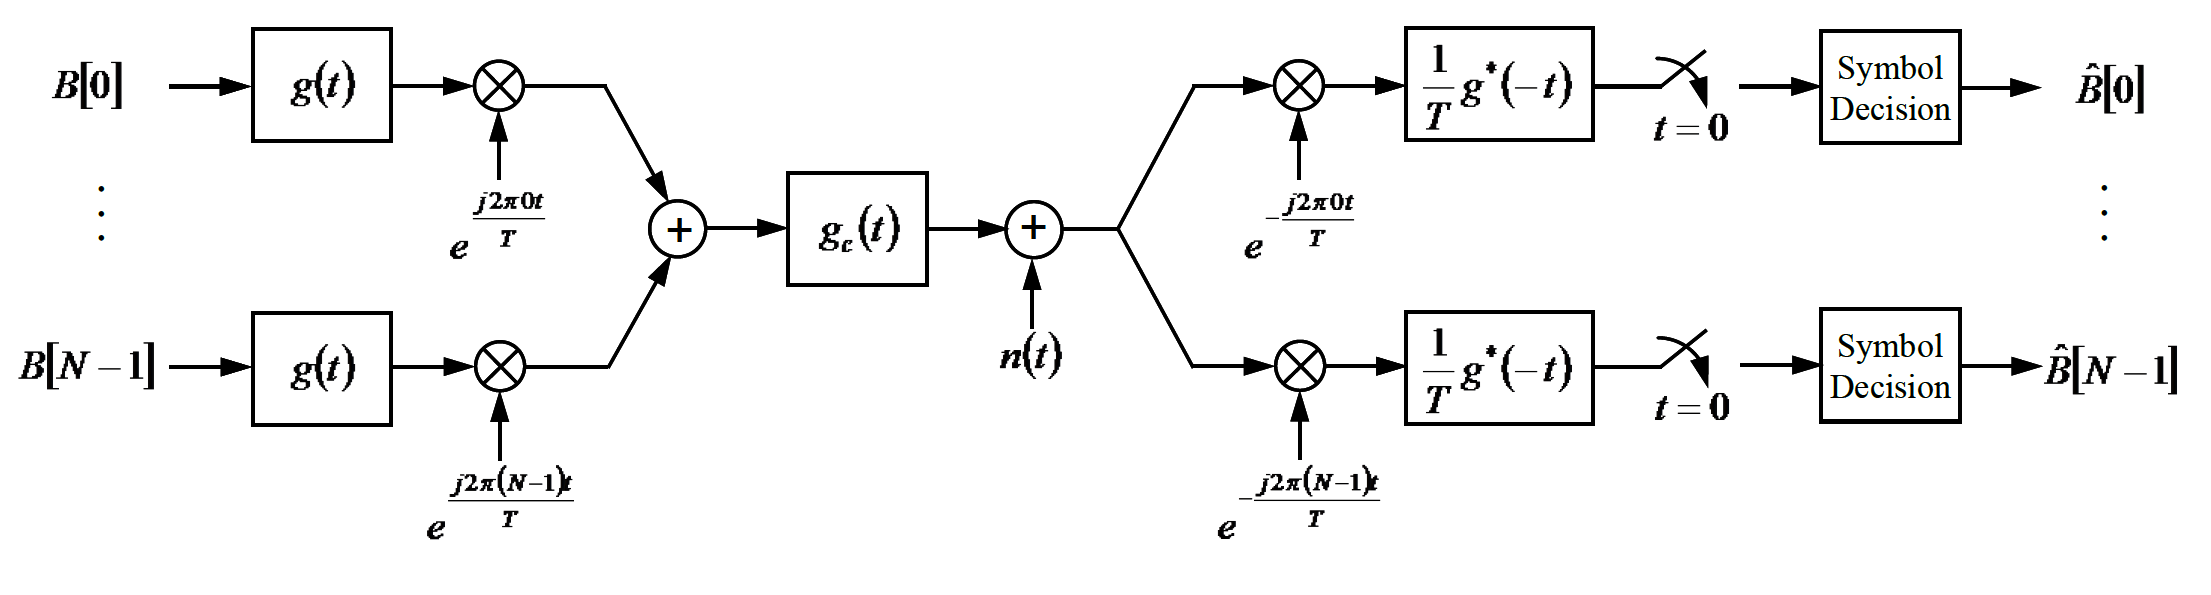
\includegraphics[scale=0.3]{figs/analog_ofdm.png}\\
	{\color{gray} \small Analog implementation of OFDM. Diagram taken from EE 379 lecture notes.}
\end{figure}

OFDM was proposed in the 60's, but making such transmission in analog electronics was impossible, since the oscillators had to be perfectly synchronize to guarantee orthogonality
\end{frame}


%
\begin{frame}{Application example: OFDM}
With the advent of the FFT, it was realized that OFDM could be implemented using the IFFT/FFT:

\begin{figure}
	\centering
	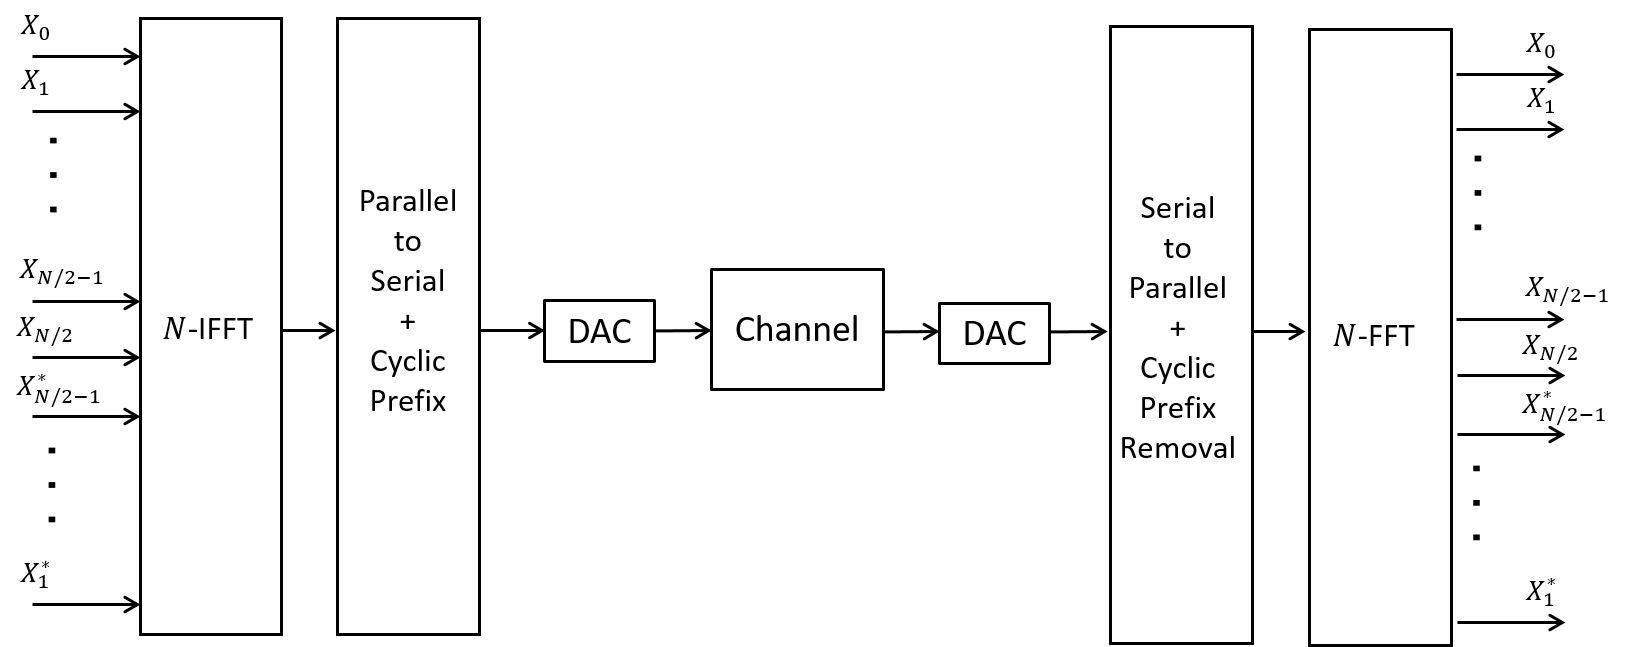
\includegraphics[scale=0.4]{figs/ofdm_diagram_fft.png}\\
	{\color{gray} \small FFT/IFFT-based implementation of OFDM.}
\end{figure}


OFDM is used in
\begin{itemize}
	\item \textbf{Long-term evolution (LTE)}, IFFT/FFT size up to 2048
	\item \textbf{Wi-Fi}, IFFT/FFT size up to 256
	\item \textbf{Bluetooth}
\end{itemize} 
\end{frame}

% 
\begin{frame}{FFT algorithms}
	FFT algorithms achieve dramatic reduction in computation by
	\begin{enumerate}
		\item Exploiting the \textbf{periodicity} and \textbf{symmetry} of complex exponentials $W^{kn}$:
		\begin{align*}
		W_N^{k(N-n)} &= W_N^{-kn} = (W_N^{kn})^* \tag{complex conjugate symmetry} \\
		W_N^{kn} &= W_N^{k(n+N)} = W_N^{(k+N)n}  \tag{periodicity in $n$ and $k$}
		\end{align*}
		\item Decomposing the computation into successively smaller DFTs. 
		\begin{itemize}
			\item Decomposition of $x[n]$ into successively smaller subsequences is called \textbf{decimation in time}.
			\item Decomposition of $X[k]$ into successively smaller subsequences is called \textbf{decimation in frequency}. 
			\item The flow graph of decimation-in-frequency decomposition can be obtained by \textbf{transposing} the flow graph of decimation-in-time decomposition, and vice-versa. 
		\end{itemize}
	\end{enumerate}
\end{frame}

% 
\begin{frame}{Decimation-in-time decomposition}
Flow graph of complete decimation-in-time decomposition of an 8-point DFT computation.

The red rectangle represents a 2-point DFT.
\begin{center}
	\begin{tikzpicture}
		\node (img) {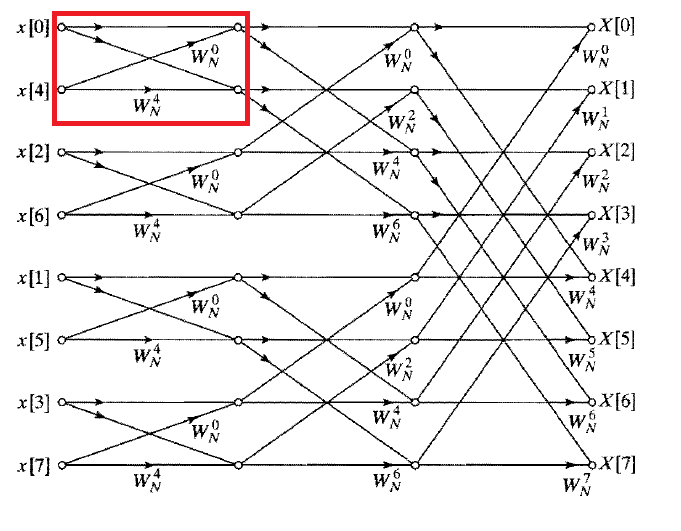
\includegraphics[scale=0.65]{figs/decimation_in_time.png}};
	\end{tikzpicture}
\end{center}

\end{frame}

% 
\begin{frame}{Decimation-in-time decomposition}
Flow graph of complete decimation-in-time decomposition of an 8-point DFT computation.

The red rectangle represents a 2-point DFT, now computed with just one multiplication by exploiting the periodicity and symmetry of $W_N^{kn}$. 
\begin{center}
	\begin{tikzpicture}
		\node (img) {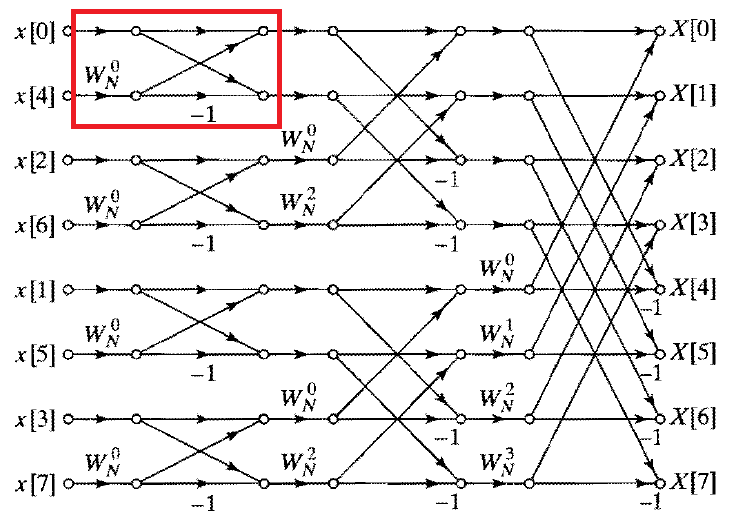
\includegraphics[scale=0.65]{figs/decimation_in_frequency.png}};
	\end{tikzpicture}
\end{center}
\end{frame}

% 
\begin{frame}{FFT algorithms}
	FFT generalizations
	\begin{itemize}
		\item Radix $R$-algorithms
		\begin{equation*}
			N = R^\nu
		\end{equation*}
		DFTs are broken into factors of $R$
		
		\item Mixed-radix algorithms
		\begin{equation*}
			N = N_1N_2\ldots N_\nu
		\end{equation*}
		DFTs are broken into factors of $\{N_1, N_2, \ldots, N_\nu\}$.
		
		\item Prime-factor algorithms
		\begin{equation*}
			N = N_1N_2\ldots N_\nu
		\end{equation*}
		DFTs are broken into prime factors $\{N_1, N_2, \ldots, N_\nu\}$.
\end{itemize}
\vspace{0.25cm}
For more detailed information on FFT algorithms see Chapter 9 of the textbook.

\vspace{0.25cm}
For open-source implementation of FFT, see \href{http://www.fftw.org/}{the Fastest Fourier Transform in the West (FFTW)}. FFTW is used in Matlab.
\end{frame}

\begin{frame}{FFT and IFFT in Matlab}
	\textbf{Useful commands:}
	
	Compute the $N$-point DFT of the vector \texttt{x}. If \texttt{N} is not passed, Matlab assumes \texttt{N = length(x)}.
	\begin{equation*}
		\texttt{>> X = fft(x, N)}
	\end{equation*}
		
	Compute the $N$-point inverse DFT of the vector \texttt{X}. If \texttt{N} is not passed, Matlab assumes \texttt{N = length(X)}.
	\begin{equation*}
	\texttt{>> x = ifft(X, N)}
	\end{equation*}
	
	To obtain the $N$-point DFT for frequencies in $[-\pi, \pi)$
	\begin{equation*}
	\texttt{>> fftshift(X)}
	\end{equation*}
	
	To restore the $N$-point DFT for frequencies in $[0, 2\pi)$
	\begin{equation*}
	\texttt{>> ifftshift(X)}
	\end{equation*}
	
\end{frame}

%
\section{Properties of the DFT}
\begin{frame}{Outline}
	\tableofcontents[currentsection]
\end{frame}
\begin{frame}{Properties of the DFT}
	\begin{itemize}
		\item The DFT shares many properties with the DTFT and with the $z$-transform
		\item However, since the DFT is periodic in time and frequency, most properties will appear in a \textit{circular} form
		\item For this reason, it is convenient to define a notation for \textbf{circular indexing}:
		\begin{equation*}
			((n))_N \equiv n~\text{modulo}~N
		\end{equation*}
		\textbf{Examples:} $X[0] = X[((7))_7]$, $X[1] = X[((6))_5]$, $X[8] = X[((17))_9]$.
		
		\item A complete list of properties is given in Table 8.2 of the textbook DTSP. This table is shown in the next slide
		\item We will cover in detail the circular time shift and circular convolution properties
	\end{itemize}
\end{frame}

%
\begin{frame}{Properties of the DFT}
	\centering
	\resizebox{!}{0.85\textheight}{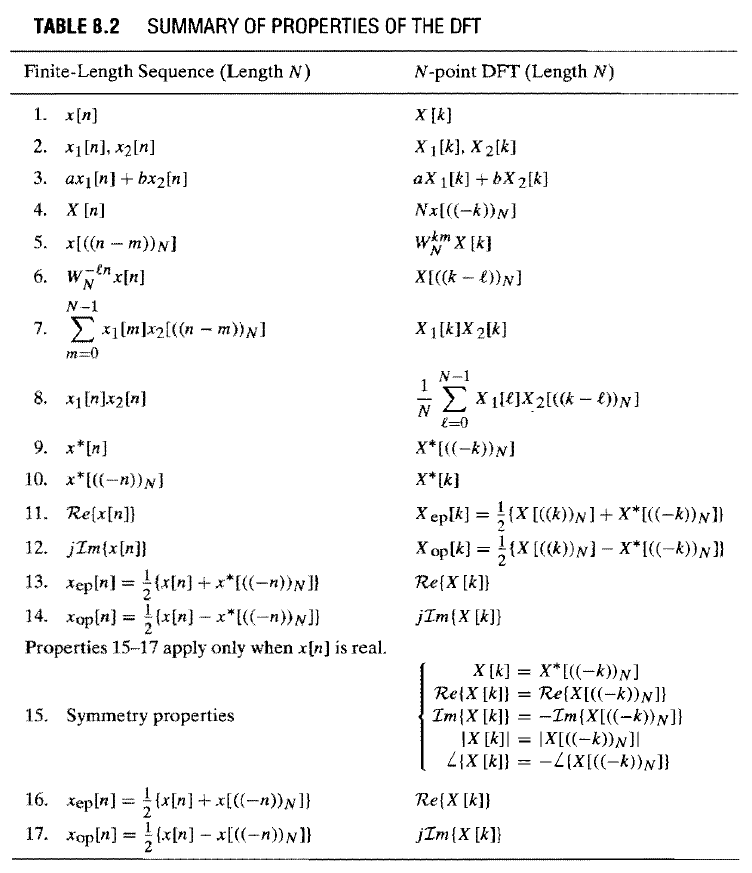
\includegraphics{figs/dft_properties_table.png}}
\end{frame}

%
\begin{frame}{Circular time shift}
\begin{equation*}
	x[((n-m))_N] \Longleftrightarrow W_N^{km}X[k] \tag{circular time shift}
\end{equation*}

To understand circular time shift and other properties of the DFT, it is useful to work with the periodic extension of $x[n]$, $\tilde{x}[n]$

\begin{center}
	\resizebox{0.8\textwidth}{!}{% \N and \Ns must be defined before calling this picture.
\def\N{5}
\def\Ns{10}
\begin{tikzpicture}
\begin{axis}[
	name=plot1a,
	axis y line=middle, axis x line=bottom,
	enlargelimits = false, clip=true,
	scale only axis,
	width=0.7\textwidth,
	height=0.3\textwidth,
	ymin=0,	ymax=1.1,
	xmin={-5}, xmax={15},
	axis line style={->,>=stealth},
	y axis line style={draw=none},
	x axis line style={shorten >= -0.25cm}, 
	xlabel={\large $n$},
	ylabel={\large $\tilde{x}[n]$},
	every axis x label/.style={
		at={(ticklabel* cs:1)},
		xshift=0.25cm,
		anchor=north,
	},
	every axis y label/.style={
		at={(ticklabel* cs:0.95)},
		anchor=south,
		xshift=0.6cm,
	},
	xtick={0, 9},
	xticklabels={0, $N-1$},
	xticklabel style={xshift=-0.15cm, yshift=-0.1cm},
	ytick=\empty,
	every outer y axis line/.append style={white!15!black},
	every y tick label/.append style={font=\color{white!15!black}},
	legend style={draw=white!15!black,fill=white,legend cell align=left}]
	\addplot[ycomb, mark=*, fill=white, mark options={scale=1.5, fill=white}, line width=1.5pt, domain=-\Ns-\N:\Ns+\N, samples=2*(\Ns+\N)+1] {triang(x+2*\Ns-\N, \N) + triang(x-\N, \N) + triang(x-\N-\Ns, \N) + triang(x-\N+\Ns, \N)};
\end{axis}

\begin{axis}[
	name=plot1b,
	at= (plot1a.east), anchor=west, xshift=3cm,
	axis y line=middle, axis x line=bottom,
	enlargelimits = false, clip=true,
	scale only axis,
	width=0.7\textwidth,
	height=0.3\textwidth,
	ymin=0,	ymax=1.1,
	y axis line style={draw=none},
	xmin={-5}, xmax={15},
	axis line style={->,>=stealth},
	x axis line style={shorten >= -0.25cm}, 
	xlabel={\large $n$},
	ylabel={\large $\tilde{x}[n-m]$},
	every axis x label/.style={
		at={(ticklabel* cs:1)},
		xshift=0.25cm,
		anchor=north,
	},
	every axis y label/.style={
		at={(ticklabel* cs:0.95)},
		anchor=south,
		xshift=1cm,
	},
	xtick={0, 4, 9},
	xticklabels={0, $m$, $N-1$},
	xticklabel style={xshift=-0.15cm, yshift=-0.1cm},
	ytick=\empty,
	every outer y axis line/.append style={white!15!black},
	every y tick label/.append style={font=\color{white!15!black}},
	legend style={draw=white!15!black,fill=white,legend cell align=left}]
		
	\addplot[ycomb, mark=*, fill=white, mark options={scale=1.5, fill=white}, line width=1.5pt, domain=-\Ns-\N:\Ns+\N, samples=2*(\Ns+\N)+1] {triang(x-4+2*\Ns-\N, \N) + triang(x-4-\N, \N) + triang(x-4-\Ns-\N, \N) + triang(x-4+\Ns-\N, \N)};
\end{axis}

\draw[->, ultra thick, shorten >= 0.2cm, shorten <= 0.2cm] (plot1a.east) to (plot1b.west);
\node[above=0.25cm, align=center, text width=3.5cm]  at ($(plot1a.east)!0.55!(plot1b.west)$) {\Large Time-shift by $m$};

\begin{axis}[
	name=plot2a,
	at=(plot1a.below south east), anchor=above north east,
	axis y line=middle, axis x line=bottom,
	enlargelimits = false, clip=true,
	scale only axis,
	width=0.7\textwidth,
	height=0.3\textwidth,
	ymin=0,	ymax=1.1,
	xmin={-5}, xmax={15},
	axis line style={->,>=stealth},
	y axis line style={draw=none},
	x axis line style={shorten >= -0.25cm}, 
	xlabel={\large $n$},
	ylabel={\large $x[n]$},
	every axis x label/.style={
		at={(ticklabel* cs:1)},
		xshift=0.25cm,
		anchor=north,
	},
	every axis y label/.style={
		at={(ticklabel* cs:0.95)},
		anchor=south,
		xshift=0.6cm,
	},
	xtick={0, 9},
	xticklabels={0, $N-1$},
	xticklabel style={xshift=-0.15cm, yshift=-0.1cm},
	ytick=\empty,
	every outer y axis line/.append style={white!15!black},
	every y tick label/.append style={font=\color{white!15!black}},
	legend style={draw=white!15!black,fill=white,legend cell align=left}]
	\addplot[ycomb, mark=*, fill=white, mark options={scale=1.5, fill=white}, line width=1.5pt, domain=-\Ns-\N:\Ns+\N, samples=2*(\Ns+\N)+1] {triang(x-\N, \N)};
\end{axis}

\begin{axis}[
	name=plot2b,
	at= (plot2a.east), anchor=west, xshift=3cm,
	axis y line=middle, axis x line=bottom,
	enlargelimits = false, clip=true,
	scale only axis,
	width=0.7\textwidth,
	height=0.3\textwidth,
	ymin=0,	ymax=1.1,
	xmin={-5}, xmax={15},
	axis line style={->,>=stealth},
	y axis line style={draw=none},
	x axis line style={shorten >= -0.25cm}, 
	xlabel={\large $n$},
	ylabel={\large $x[((n-m))_N]$},
	every axis x label/.style={
		at={(ticklabel* cs:1)},
		xshift=0.25cm,
		anchor=north,
	},
	every axis y label/.style={
		at={(ticklabel* cs:0.95)},
		anchor=south,
		xshift=1.5cm,
	},
	xtick={0, 4, 9},
	xticklabels={0, $m$, $N-1$},
	xticklabel style={xshift=-0.15cm, yshift=-0.1cm},
	ytick=\empty,
	every outer y axis line/.append style={white!15!black},
	every y tick label/.append style={font=\color{white!15!black}},
	legend style={draw=white!15!black,fill=white,legend cell align=left}]
	
	\addplot[ycomb, mark=*, fill=white, mark options={scale=1.5, fill=white}, line width=1.5pt, domain=0:\Ns-1, samples=\Ns] {triang(x-4-\N, \N) + triang(x-4-\N+\Ns, \N) };
	\addplot[ycomb, mark=*, fill=white, mark options={scale=1.5, fill=white}, line width=1.5pt, domain=-\Ns:-1, samples=\Ns-1] {0};
	\addplot[ycomb, mark=*, fill=white, mark options={scale=1.5, fill=white}, line width=1.5pt, domain=\Ns:2*\Ns-1, samples=\Ns] {0};
\end{axis}

\draw[->, ultra thick, shorten >= 0.2cm, shorten <= -0.4cm] (plot2a.east) to (plot2b.west);
\node[above=0.25cm, , align=center, text width=4cm]  at ($(plot2a.east)!0.5!(plot2b.west)$) {\Large Circular-shift by $m$};

\draw[red2, dashed, very thick] ($(plot1a.north)-(1.9cm, -0.75cm)$) to ($(plot2a.south)-(1.9cm, 0.75cm)$);
\draw[red2, dashed, very thick] ($(plot1a.north)+(1.5cm, 0.75cm)$) to ($(plot2a.south)+(1.5cm, -0.75cm)$);
\draw[red2, dashed, very thick] ($(plot1b.north)-(1.9cm, -0.75cm)$) to ($(plot2b.south)-(1.9cm, 0.75cm)$);
\draw[red2, dashed, very thick] ($(plot1b.north)+(1.5cm, 0.75cm)$) to ($(plot2b.south)+(1.5cm, -0.75cm)$);

\end{tikzpicture}
}
\end{center}
\end{frame}

%
\begin{frame}{Circular convolution}
	Product in the frequency domain means \textbf{circular convolution} in time domain
	\begin{equation*}
		x[n]~\encircle{N}~y[n] = \sum_{m=0}^{N-1} x[m]y[((n-m))_N] \Longleftrightarrow X[k]Y[k] \tag{circular convolution in time}
	\end{equation*}
	
	Similarly, product in time domain means \textbf{circular convolution} in frequency domain
	
	\begin{equation*}
	x[n]y[n] \Longleftrightarrow X[k]~\encircle{N}~Y[k] = \sum_{m=0}^{N-1} X[m]Y[((k-m))_N] \tag{circular convolution in frequency}
	\end{equation*}
\end{frame}

%
\begin{frame}{Understanding circular convolution}
	\begin{center}
		\resizebox{0.5\textwidth}{!}{% \N and \Ns must be defined before calling this picture.
\def\N{5}
\def\Ns{10}
\begin{tikzpicture}
\begin{axis}[
	name=plot1,
	axis y line=middle, axis x line=bottom,
	enlargelimits = upper, clip=true,
	scale only axis,
	width=\textwidth,
	height=0.2\textwidth,
	ymin=0,	ymax=1.1,
	xmin={0}, xmax={15},
	axis line style={->,>=stealth},
	%y axis line style={draw=none},
	x axis line style={shorten >= -0.25cm}, 
	xlabel={\large $n$},
	ylabel={\large $x[n]$},
	every axis x label/.style={
		at={(ticklabel* cs:1)},
		xshift=0.25cm,
		anchor=north,
	},
	every axis y label/.style={
		at={(ticklabel* cs:0.95)},
		anchor=south,
		xshift=0.6cm,
	},
	xtick={0, 9},
	xticklabels={0, $L-1$},
	%xticklabel style={xshift=-0.15cm, yshift=-0.1cm},
	ytick={1},
	every outer y axis line/.append style={white!15!black},
	every y tick label/.append style={font=\color{white!15!black}},
	legend style={draw=white!15!black,fill=white,legend cell align=left}]
	%\addplot[ycomb, mark=*, fill=white, mark options={scale=1.5, fill=white}, line width=1.5pt, domain=-\Ns-\N:\Ns+\N, samples=2*(\Ns+\N)+1] {triang(x+2*\Ns-\N, \N) + triang(x-\N, \N) + triang(x-\N-\Ns, \N) + triang(x-\N+\Ns, \N)};
	\addplot[ycomb, mark=*, fill=white, mark options={scale=1.5, fill=white}, line width=1.5pt, domain=0:\Ns-1, samples=\Ns] {triang(x-\N, \N)};
	\node[fill=black!20, text width=1.5cm, align=center, inner sep=2mm, anchor=south west] at (axis cs: 9, 0.5) {Length $L$};
\end{axis}

\begin{axis}[
	name=plot2,
	at=(plot1.below south east), anchor=above north east,
	axis y line=middle, axis x line=bottom,
	enlargelimits = upper, clip=true,
	scale only axis,
	width=\textwidth,
	height=0.2\textwidth,
	ymin=0,	ymax=1.1,
	%y axis line style={draw=none},
	xmin={0}, xmax={15},
	axis line style={->,>=stealth},
	x axis line style={shorten >= -0.25cm}, 
	xlabel={\large $n$},
	ylabel={\large $y[n]$},
	every axis x label/.style={
		at={(ticklabel* cs:1)},
		xshift=0.25cm,
		anchor=north,
	},
	every axis y label/.style={
		at={(ticklabel* cs:1)},
		anchor=south,
		xshift=0.6cm,
	},
	xtick={0, 4, 9},
	xticklabels={0, $P-1$, $L-1$},
	%xticklabel style={xshift=-0.15cm, yshift=-0.1cm},
	ytick={1},
	every outer y axis line/.append style={white!15!black},
	every y tick label/.append style={font=\color{white!15!black}},
	legend style={draw=white!15!black,fill=white,legend cell align=left}]
		
	\addplot[ycomb, mark=*, fill=white, mark options={scale=1.5, fill=white}, line width=1.5pt, domain=0:\Ns-1, samples=\Ns] {rect(x, \N)};
	\node[fill=black!20, text width=1.5cm, align=center, inner sep=2mm, anchor=south west] at (axis cs: 9, 0.5) {Length $P$};
\end{axis}

\onslide<2-|handout:1->{
\begin{axis}[
name=plot3,
at=(plot2.below south east), anchor=above north east,
axis y line=middle, axis x line=bottom,
enlargelimits = upper, clip=true,
scale only axis,
width=\textwidth,
height=0.2\textwidth,
ymin=0,	ymax=4,
%y axis line style={draw=none},
xmin={0}, xmax={15},
axis line style={->,>=stealth},
x axis line style={shorten >= -0.25cm}, 
xlabel={\large $n$},
ylabel={\large $x[n]\ast y[n]$},
every axis x label/.style={
	at={(ticklabel* cs:1)},
	xshift=0.25cm,
	anchor=north,
},
every axis y label/.style={
	at={(ticklabel* cs:1)},
	anchor=south,
	xshift=0.6cm,
},
xtick={0, 9, 13},
xticklabels={0, $L-1$, $L+P-2$},
%xticklabel style={xshift=-0.15cm, yshift=-0.1cm},
ytick={3.8},
every outer y axis line/.append style={white!15!black},
every y tick label/.append style={font=\color{white!15!black}},
legend style={draw=white!15!black,fill=white,legend cell align=left}]

\addplot[ycomb, mark=*, fill=white, mark options={scale=1.5, fill=white}, line width=1.5pt] 
table[row sep=crcr]{
	%-5 0\\
	%-4 0\\
	%-3 0\\
	%-2 0\\
	%-1 0\\
	0 0 \\ 
	1 0.2 \\
	2 0.6 \\
	3 1.2 \\
	4 2 \\
	5 3 \\
	6 3.6 \\
	7 3.8 \\
	8 3.6 \\
	9 3 \\
	10 2 \\
	11 1.2 \\
	12 0.6 \\
	13 0.2 \\
	%14 0 \\
	%15 0 \\
	%16 0 \\
	%17 0 \\
	%18 0 \\
	%19 0 \\
	%20 0 \\
};
\node[align=center, text width=2cm, inner sep=2mm, fill=black!20, anchor=south west] at (axis cs: 10, 2.5) {Linear convolution};
\end{axis}
}


\onslide<3-|handout:1->{
	\begin{axis}[
	name=plot4,
	at=(plot3.below south east), anchor=above north east,
	axis y line=middle, axis x line=bottom,
	enlargelimits = upper, clip=true,
	scale only axis,
	width=\textwidth,
	height=0.2\textwidth,
	ymin=0,	ymax=4,
	%y axis line style={draw=none},
	xmin={0}, xmax={15},
	axis line style={->,>=stealth},
	x axis line style={shorten >= -0.25cm}, 
	xlabel={\large $n$},
	ylabel={\large $x[n]~\encircle{N}~y[n]$},
	every axis x label/.style={
		at={(ticklabel* cs:1)},
		xshift=0.25cm,
		anchor=north,
	},
	every axis y label/.style={
		at={(ticklabel* cs:1)},
		anchor=south,
		xshift=0.6cm,
	},
	xtick={0, 3, 9},
	xticklabels={0, $P-2$, $L-1$},
	%xticklabel style={xshift=-0.15cm, yshift=-0.1cm},
	ytick={3.8},
	every outer y axis line/.append style={white!15!black},
	every y tick label/.append style={font=\color{white!15!black}},
	legend style={draw=white!15!black,fill=white,legend cell align=left}]
	
	\only<3|handout:1>{
	\addplot[ycomb, mark=*, fill=white, mark options={scale=1.5, fill=white}, line width=1.5pt] 
	table[row sep=crcr]{
		0 0 \\ 
		1 0.2 \\
		2 0.6 \\
		3 1.2 \\
		4 2 \\
		5 3 \\
		6 3.6 \\
		7 3.8 \\
		8 3.6 \\
		9 3 \\
	};

	\addplot[ycomb, blue2!40, mark=*, fill=white, mark options={scale=1.5, fill=white}, line width=1.5pt] 
	table[row sep=crcr]{
		10 2 \\
		11 1.2 \\
		12 0.6 \\
		13 0.2 \\
	};

	\addplot[ycomb, blue2, mark=*, fill=white, mark options={scale=1.5, fill=white}, line width=1.5pt] 
	table[row sep=crcr]{
		0 2 \\
		1 1.2 \\
		2 0.6 \\
		3 0.2 \\
	};
	}


	\only<4|handout:2>{
		\addplot[ycomb, red2, mark=*, fill=white, mark options={scale=1.5, fill=white}, line width=1.5pt] 
		table[row sep=crcr]{
			0 2 \\
			1 1.4 \\
			2 1.2 \\
			3 1.4 \\
			4 2 \\
			5 3 \\
			6 3.6 \\
			7 3.8 \\
			8 3.6 \\
			9 3 \\
		};
		\node[align=center, text width=3cm, inner sep=2mm, fill=black!20, anchor=south west] at (axis cs: 10, 1.5) {$N$-point circular convolution \\
		$N = L$};
	}


\end{axis}
}
\end{tikzpicture}	
}
	\end{center}
\end{frame}

\begin{frame}{Understanding circular convolution}
In this first example
\begin{itemize}
	\item $x[n]$ has length $L$, while $y[n]$ has length $P$
	\item The result of linear convolution $x[n]\ast [y]$ has length $L+P-1$
	\item For the $N$-point circular convolution, the {\color{blue2} $P-1$ samples that fall beyond $N-1$} are added to the beginning of the sequence
	\item Note that the $N$-point circular convolution and the linear convolution produce different results
	\item We can make the circular convolution equal to the linear convolution by zero-padding the sequences and performing the $(L+P-1)$-point circular convolution
\end{itemize}
\end{frame}

%
\begin{frame}{Understanding circular convolution}
\begin{center}
	\resizebox{0.5\textwidth}{!}{% \N and \Ns must be defined before calling this picture.
\def\N{5}
\def\Ns{14}
\begin{tikzpicture}
\begin{axis}[
	name=plot1,
	axis y line=middle, axis x line=bottom,
	enlargelimits = upper, clip=true,
	scale only axis,
	width=\textwidth,
	height=0.2\textwidth,
	ymin=0,	ymax=1.1,
	xmin={0}, xmax={15},
	axis line style={->,>=stealth},
	%y axis line style={draw=none},
	x axis line style={shorten >= -0.25cm}, 
	xlabel={\large $n$},
	ylabel={\large $x[n]$},
	every axis x label/.style={
		at={(ticklabel* cs:1)},
		xshift=0.25cm,
		anchor=north,
	},
	every axis y label/.style={
		at={(ticklabel* cs:0.95)},
		anchor=south,
		xshift=0.6cm,
	},
	xtick={0, 9, 13},
	xticklabels={0, $L-1$, $L+P-2$},
	%xticklabel style={xshift=-0.15cm, yshift=-0.1cm},
	ytick={1},
	every outer y axis line/.append style={white!15!black},
	every y tick label/.append style={font=\color{white!15!black}},
	legend style={draw=white!15!black,fill=white,legend cell align=left}]
	%\addplot[ycomb, mark=*, fill=white, mark options={scale=1.5, fill=white}, line width=1.5pt, domain=-\Ns-\N:\Ns+\N, samples=2*(\Ns+\N)+1] {triang(x+2*\Ns-\N, \N) + triang(x-\N, \N) + triang(x-\N-\Ns, \N) + triang(x-\N+\Ns, \N)};
	\addplot[ycomb, mark=*, fill=white, mark options={scale=1.5, fill=white}, line width=1.5pt, domain=0:\Ns-1, samples=\Ns] {triang(x-\N, \N)};
	\node[fill=black!20, text width=1.5cm, align=center, inner sep=2mm, anchor=south west] at (axis cs: 9, 0.5) {Length $L$};
\end{axis}

\begin{axis}[
	name=plot2,
	at=(plot1.below south east), anchor=above north east,
	axis y line=middle, axis x line=bottom,
	enlargelimits = upper, clip=true,
	scale only axis,
	width=\textwidth,
	height=0.2\textwidth,
	ymin=0,	ymax=1.1,
	%y axis line style={draw=none},
	xmin={0}, xmax={15},
	axis line style={->,>=stealth},
	x axis line style={shorten >= -0.25cm}, 
	xlabel={\large $n$},
	ylabel={\large $y[n]$},
	every axis x label/.style={
		at={(ticklabel* cs:1)},
		xshift=0.25cm,
		anchor=north,
	},
	every axis y label/.style={
		at={(ticklabel* cs:1)},
		anchor=south,
		xshift=0.6cm,
	},
	xtick={0, 4, 9, 13},
	xticklabels={0, $P-1$, $L-1$, $L+P-2$},
	%xticklabel style={xshift=-0.15cm, yshift=-0.1cm},
	ytick={1},
	every outer y axis line/.append style={white!15!black},
	every y tick label/.append style={font=\color{white!15!black}},
	legend style={draw=white!15!black,fill=white,legend cell align=left}]
		
	\addplot[ycomb, mark=*, fill=white, mark options={scale=1.5, fill=white}, line width=1.5pt, domain=0:\Ns-1, samples=\Ns] {rect(x, \N)};
	\node[fill=black!20, text width=1.5cm, align=center, inner sep=2mm, anchor=south west] at (axis cs: 9, 0.5) {Length $P$};
\end{axis}

\onslide<2-|handout:1->{
\begin{axis}[
name=plot3,
at=(plot2.below south east), anchor=above north east,
axis y line=middle, axis x line=bottom,
enlargelimits = upper, clip=true,
scale only axis,
width=\textwidth,
height=0.2\textwidth,
ymin=0,	ymax=4,
%y axis line style={draw=none},
xmin={0}, xmax={15},
axis line style={->,>=stealth},
x axis line style={shorten >= -0.25cm}, 
xlabel={\large $n$},
ylabel={\large $x[n]\ast y[n]$},
every axis x label/.style={
	at={(ticklabel* cs:1)},
	xshift=0.25cm,
	anchor=north,
},
every axis y label/.style={
	at={(ticklabel* cs:1)},
	anchor=south,
	xshift=0.6cm,
},
xtick={0, 9, 13},
xticklabels={0, $L-1$, $L+P-2$},
%xticklabel style={xshift=-0.15cm, yshift=-0.1cm},
ytick={3.8},
every outer y axis line/.append style={white!15!black},
every y tick label/.append style={font=\color{white!15!black}},
legend style={draw=white!15!black,fill=white,legend cell align=left}]

\addplot[ycomb, mark=*, fill=white, mark options={scale=1.5, fill=white}, line width=1.5pt] 
table[row sep=crcr]{
	%-5 0\\
	%-4 0\\
	%-3 0\\
	%-2 0\\
	%-1 0\\
	0 0 \\ 
	1 0.2 \\
	2 0.6 \\
	3 1.2 \\
	4 2 \\
	5 3 \\
	6 3.6 \\
	7 3.8 \\
	8 3.6 \\
	9 3 \\
	10 2 \\
	11 1.2 \\
	12 0.6 \\
	13 0.2 \\
	%14 0 \\
	%15 0 \\
	%16 0 \\
	%17 0 \\
	%18 0 \\
	%19 0 \\
	%20 0 \\
};
\node[align=center, text width=2cm, inner sep=2mm, fill=black!20, anchor=south west] at (axis cs: 10, 2.5) {Linear convolution};
\end{axis}
}


\onslide<3-|handout:1->{
	\begin{axis}[
	name=plot4,
	at=(plot3.below south east), anchor=above north east,
	axis y line=middle, axis x line=bottom,
	enlargelimits = upper, clip=true,
	scale only axis,
	width=\textwidth,
	height=0.2\textwidth,
	ymin=0,	ymax=4,
	%y axis line style={draw=none},
	xmin={0}, xmax={15},
	axis line style={->,>=stealth},
	x axis line style={shorten >= -0.25cm}, 
	xlabel={\large $n$},
	ylabel={\large $x[n]~\encircle{N}~y[n]$},
	every axis x label/.style={
		at={(ticklabel* cs:1)},
		xshift=0.25cm,
		anchor=north,
	},
	every axis y label/.style={
		at={(ticklabel* cs:1)},
		anchor=south,
		xshift=0.6cm,
	},
	xtick={0, 9, 13},
	xticklabels={0, $L-1$, $L+P-2$},
	%xticklabel style={xshift=-0.15cm, yshift=-0.1cm},
	ytick={3.8},
	every outer y axis line/.append style={white!15!black},
	every y tick label/.append style={font=\color{white!15!black}},
	legend style={draw=white!15!black,fill=white,legend cell align=left}]
	
	\addplot[ycomb, mark=*, fill=white, mark options={scale=1.5, fill=white}, line width=1.5pt] 
	table[row sep=crcr]{
		0 0 \\ 
		1 0.2 \\
		2 0.6 \\
		3 1.2 \\
		4 2 \\
		5 3 \\
		6 3.6 \\
		7 3.8 \\
		8 3.6 \\
		9 3 \\
	};

	\addplot[ycomb, black, mark=*, fill=white, mark options={scale=1.5, fill=white}, line width=1.5pt] 
	table[row sep=crcr]{
		10 2 \\
		11 1.2 \\
		12 0.6 \\
		13 0.2 \\
	};


	\node[align=center, text width=3cm, inner sep=2mm, fill=black!20, anchor=south west] at (axis cs: 11, 1.5) {$N$-point circular convolution \\
	$N = L+P-1$};
\end{axis}
}
\end{tikzpicture}	
}
\end{center}
\end{frame}

\begin{frame}{Linear convolution using circular convolution}
By zero-padding and performing the $(L+P-1)$-point circular convolution, we can calculate the linear convolution using the DFT

\vspace{0.25cm}
In Matlab:\\
The vector \texttt{x} has length $L$ while \texttt{y} has length $P$
\begin{equation*}
	\texttt{>> conv(x, y, `full')} \tag{linear convolution}
\end{equation*}

This will produce an output of length $N = L+P-1$. The linear convolution has complexity $\mathcal{O}(N^2)$

\begin{equation*}
\texttt{>> ifft(fft(x, N).*fft(y, N))} \tag{circular convolution}
\end{equation*}

The parameter \texttt{N} tells Matlab to zero-pad vectors \texttt{x} and \texttt{y}  and compute the $N$-point DFT. The FFT/IFFT has complexity $\mathcal{O}(N\log N)$

\vspace{0.25cm}
\textbf{Conclusion:} for $N$ large, it is more efficient to compute the linear convolution through the DFT using FFT algorithm.
\end{frame}

\section{Block convolution}
\begin{frame}{Linear convolution using circular convolution}

	Recall that for FIR filters, filtering is essentially a linear convolution between the input and the filter coefficients:
	\begin{equation*}
		y[n] = x[n] \ast h[n] = \sum_{m =0}^{M} h[m]x[n-m]
	\end{equation*}
	where $M$ is the filter order.
	
	\vspace{0.25cm}
	We can implement this filter using the DFT:
	\begin{center}
		\resizebox{0.7\textwidth}{!}{\begin{tikzpicture}[->, >=stealth, shorten >= 0pt, draw=black!50, node distance=2cm, font=\sffamily]
    \tikzstyle{node}=[circle,fill=black,minimum size=2pt,inner sep=0pt]
    \tikzstyle{block}=[draw=black,rectangle,fill=none,minimum size=1cm, inner sep=0pt]
    \tikzstyle{adder}=[draw=black,circle,fill=none,minimum size=0.75cm, inner sep=0pt]

	\node[node] (xc) at (0, 0) {};
    \node[block, right=1cm of xc] (fft) {FFT};
    \node[adder, right of=fft] (mult) {\Large $\times$};
    \node[block, right of=mult] (ifft) {IFFT};
    \node[node, below=1cm of mult] (h) {};
	\coordinate[right=1cm of ifft] (yc) {};
	
	\coordinate (mid1) at ($(fft.east)!0.5!(mult.west)$) {};
	\coordinate (mid2) at ($(mult.east)!0.5!(ifft.west)$) {};
		
    \path (xc) edge (fft);
    \path (fft) edge (mult);
    \path (mult) edge (ifft);
    \path (h) edge (mult.south);
    \path (ifft) edge (yc);
    
    \node[above = 0.5mm of mid1] {$X[k]$};
    \node[above = 0.5mm of mid2] {$Y[k]$};
    \node[above = 0mm of xc, text width = 1cm, align=center] {$x[n]$};
    \node[above = 0mm of yc, text width = 1cm, align=center] {$y[n]$};
    \node[right = 0mm of h, text width = 3cm, align=center] {$H[k] = \mathrm{DFT}\{h[n]\}$};
    

\end{tikzpicture}}
	\end{center}

	By using \textbf{block convolution} we process the samples in batches.
	\begin{enumerate}
		\item Overlap-add method
		\item Overlap-save method
	\end{enumerate}
\end{frame}


\begin{frame}{Overlap-add method}
In the \textbf{overlap-add method} the incoming signal $x[n]$ is broken down into several \underline{non-overlapping} segments $x_r[n]$, each of length $L$:
\begin{equation*}
	x_r[n] = \begin{cases}
	x[n + rL], & 0 \leq n \leq L-1\\
	0, & \text{otherwise}
	\end{cases}
\end{equation*}

For each segment, we compute the $N$-point circular convolution of $x_r[n]$ and the filter impulse response $h[n]$:

\begin{equation*}
	y_r[n] = h[n]~\encircle{N}~x_r[n] = h[n]\ast x_r[n]
\end{equation*}
where $N \geq L + M$ so that $y_r[n]$ is equivalent to the linear convolution of $x_r[n]$ and $h[n]$. Note that $M$ is the filter order. Hence, the filter has \underline{$M+1$ coefficients}.

Finally, the output is computed by adding the filtered segments
\begin{equation*}
	y_r[n] = \sum_{r = 0}^{\infty} y_r[n - rL]
\end{equation*}
The sequences $y_r[n-rL]$ overlap by $M$ samples.
\end{frame}

%
\begin{frame}{Overlap-add method}
\begin{center}
	\resizebox{0.62\textwidth}{!}{% \N and \Ns must be defined before calling this picture.
\def\N{5}
\def\Ns{10}
\begin{tikzpicture}
\begin{axis}[
	name=plot1,
	axis y line=middle, axis x line=bottom,
	enlargelimits = upper, clip=true,
	scale only axis,
	width=\textwidth,
	height=0.2\textwidth,
	ymin=0,	ymax=1.1,
	xmin={0}, xmax={44},
	axis line style={->,>=stealth},
	%y axis line style={draw=none},
	x axis line style={shorten >= -0.25cm}, 
	xlabel={\large $n$},
	ylabel={\large $h[n]$},
	every axis x label/.style={
		at={(ticklabel* cs:1)},
		xshift=0.25cm,
		anchor=north,
	},
	every axis y label/.style={
		at={(ticklabel* cs:0.95)},
		anchor=south,
		xshift=0.6cm,
	},
	xtick={0, 9},
	xticklabels={0, $M$},
	%xticklabel style={xshift=-0.15cm, yshift=-0.1cm},
	ytick={1},
	every outer y axis line/.append style={white!15!black},
	every y tick label/.append style={font=\color{white!15!black}},
	legend style={draw=white!15!black,fill=white,legend cell align=left}]
	%\addplot[ycomb, mark=*, fill=white, mark options={scale=1.5, fill=white}, line width=1.5pt, domain=-\Ns-\N:\Ns+\N, samples=2*(\Ns+\N)+1] {triang(x+2*\Ns-\N, \N) + triang(x-\N, \N) + triang(x-\N-\Ns, \N) + triang(x-\N+\Ns, \N)};
	\addplot[ycomb, mark=*, fill=white, mark options={scale=1.5, fill=white}, line width=1.5pt, domain=0:\Ns-1, samples=\Ns] {triang(x-\N, \N)};
	\node[fill=black!20, text width=3cm, align=center, inner sep=2mm, anchor=south west] at (axis cs: 10, 0.5) {Filter coefficients \\ Length $M+1$};
\end{axis}

\begin{axis}[
	name=plot2,
	at=(plot1.below south east), anchor=above north east,
	axis y line=middle, axis x line=middle,
	enlargelimits = false, clip=true,
	scale only axis,
	width=\textwidth,
	height=0.2\textwidth,
	ymin=-2,	ymax=2,
	%y axis line style={draw=none},
	xmin={0}, xmax={44},
	axis line style={->,>=stealth},
	x axis line style={shorten >= -0.25cm}, 
	xlabel={\large $n$},
	ylabel={\large $x[n]$},
	every axis x label/.style={
		at={(ticklabel* cs:1)},
		xshift=0.25cm,
		anchor=north,
	},
	every axis y label/.style={
		at={(ticklabel* cs:1)},
		anchor=south,
		xshift=0.6cm,
	},
	xtick={0},
	ytick=\empty,
	every outer y axis line/.append style={white!15!black},
	every y tick label/.append style={font=\color{white!15!black}},
	legend style={draw=white!15!black,fill=white,legend cell align=left}]
	
	\only<1|handout:0>{	
	\addplot[ycomb, mark=*, fill=white, mark options={scale=1.5, fill=white}, line width=1.5pt]
	table[row sep=crcr]{
		0 0.10491 \\
		1 0.54919 \\
		2 0.70362 \\
		3 1.0626 \\
		4 1.2488 \\
		5 1.1636 \\
		6 1.0408 \\
		7 0.9144 \\
		8 0.84567 \\
		9 0.72187 \\
		10 0.19381 \\
		11 -0.093603 \\
		12 -0.095644 \\
		13 -0.45954 \\
		14 -0.54561 \\
		15 -0.57977 \\
		16 -0.48307 \\
		17 -0.21808 \\
		18 -0.051949 \\
		19 0.22502 \\
		20 0.70008 \\
		21 0.69747 \\
		22 0.94023 \\
		23 1.311 \\
		24 1.4125 \\
		25 1.6667 \\
		26 1.7249 \\
		27 1.4084 \\
		28 1.1416 \\
		29 0.60004 \\
		30 0.30779 \\
		31 -0.0025167 \\
		32 -0.47202 \\
		33 -0.98919 \\
		34 -1.3251 \\
		35 -1.3521 \\
		36 -1.3193 \\
		37 -1.2023 \\
		38 -0.88282 \\
		39 -0.64963 \\
		40 -0.42971 \\
		41 -0.004122 \\
		42 0.43751 \\
		43 0.90842 \\
		44 1.0804 \\
	};
	}

	\only<2-4|handout:1>{	
	\addplot[ycomb, blue2, mark=*, fill=white, mark options={scale=1.5, fill=white}, line width=1.5pt]
	table[row sep=crcr]{
		0 0.10491 \\
		1 0.54919 \\
		2 0.70362 \\
		3 1.0626 \\
		4 1.2488 \\
		5 1.1636 \\
		6 1.0408 \\
		7 0.9144 \\
		8 0.84567 \\
		9 0.72187 \\
		10 0.19381 \\
		11 -0.093603 \\
		12 -0.095644 \\
		13 -0.45954 \\
		14 -0.54561 \\
	};
	\node[anchor=south west, blue2] at (axis cs: 8, 0.8) {\Large $x_1[n]$};
	\node[below, blue2] at (axis cs: 7, 0.1) {$L$ samples};
	}

	\only<3-4|handout:1>{	
	\addplot[ycomb, red2, mark=*, fill=white, mark options={scale=1.5, fill=white}, line width=1.5pt]
	table[row sep=crcr]{
		15 -0.57977 \\
		16 -0.48307 \\
		17 -0.21808 \\
		18 -0.051949 \\
		19 0.22502 \\
		20 0.70008 \\
		21 0.69747 \\
		22 0.94023 \\
		23 1.311 \\
		24 1.4125 \\
		25 1.6667 \\
		26 1.7249 \\
		27 1.4084 \\
		28 1.1416 \\
		29 0.60004 \\
	};
	\node[anchor=south west, red2] at (axis cs: 16, 0.8) {\Large $x_2[n]$};
	\node[below, red2] at (axis cs: 23, 0.1) {$L$ samples};
	}

	\only<4|handout:1>{	
	\addplot[ycomb, green2, mark=*, fill=white, mark options={scale=1.5, fill=white}, line width=1.5pt]
	table[row sep=crcr]{
		30 0.30779 \\
		31 -0.0025167 \\
		32 -0.47202 \\
		33 -0.98919 \\
		34 -1.3251 \\
		35 -1.3521 \\
		36 -1.3193 \\
		37 -1.2023 \\
		38 -0.88282 \\
		39 -0.64963 \\
		40 -0.42971 \\
		41 -0.004122 \\
		42 0.43751 \\
		43 0.90842 \\
		44 1.0804 \\
	};
	\node[anchor=south west, green2] at (axis cs: 39, -2) {\Large $x_3[n]$};
	\node[above, green2] at (axis cs: 35, 0) {$L$ samples};
	}
\end{axis}

\begin{axis}[
name=plot3,
at=(plot2.below south east), anchor=above north east,
axis y line=middle, axis x line=center,
enlargelimits = false, clip=true,
scale only axis,
width=\textwidth,
height=0.2\textwidth,
ymin=-11,	ymax=11,
%y axis line style={draw=none},
xmin={0}, xmax={44},
axis line style={->,>=stealth},
x axis line style={shorten >= -0.25cm}, 
xlabel={\large $n$},
ylabel={},
every axis x label/.style={
	at={(ticklabel* cs:1)},
	xshift=0.25cm,
	anchor=north,
},
every axis y label/.style={
	at={(ticklabel* cs:1)},
	anchor=south,
	xshift=0.6cm,
},
xtick=\empty,
ytick=\empty,
every outer y axis line/.append style={white!15!black},
every y tick label/.append style={font=\color{white!15!black}},
legend style={draw=white!15!black,fill=white,legend cell align=left}]

\only<2-4|handout:1>{
\addplot[ycomb, blue2, mark=*, fill=white, mark options={scale=1.5, fill=white}, line width=1.5pt] 
table[row sep=crcr]{
	0 0 \\
	1 0.020982 \\
	2 0.1518 \\
	3 0.42334 \\
	4 0.90742 \\
	5 1.6412 \\
	6 2.5658 \\
	7 3.4789 \\
	8 4.2934 \\
	9 4.852 \\
	10 5.0554 \\
	11 4.8532 \\
	12 4.3257 \\
	13 3.5541 \\
	14 2.5648 \\
	15 1.4274 \\
	16 0.44524 \\
	17 -0.29135 \\
	18 -0.80681 \\
	19 -0.96931 \\
	20 -0.76919 \\
	21 -0.53031 \\
	22 -0.31015 \\
	23 -0.10912 \\
}; % y1
\node[anchor=south west, blue2] at (axis cs: 1, -8) {\large $y_1 = h[n]~\encircle{N}~x_1[n]$};
}

\only<3-4|handout:1>{
\addplot[ycomb, red2, mark=*, fill=white, mark options={scale=1.5, fill=white}, line width=1.5pt] 
table[row sep=crcr]{
	15 0 \\
	16 -0.11595 \\
	17 -0.32852 \\
	18 -0.58471 \\
	19 -0.85128 \\
	20 -1.0729 \\
	21 -0.9225 \\
	22 -0.43942 \\
	23 0.31893 \\
	24 1.3603 \\
	25 2.5941 \\
	26 3.7653 \\
	27 4.9059 \\
	28 5.9084 \\
	29 6.6045 \\
	30 6.9006 \\
	31 6.67 \\
	32 5.8889 \\
	33 4.7325 \\
	34 3.3817 \\
	35 2.0733 \\
	36 1.0983 \\
	37 0.46833 \\
	38 0.12001 \\
}; %y2
\node[anchor=south west, red2] at (axis cs: 18, -8) {\large $y_2 = h[n]~\encircle{N}~x_2[n]$};
}

\only<4-|handout:1>{
\addplot[ycomb, green2, mark=*, fill=white, mark options={scale=1.5, fill=white}, line width=1.5pt] 
table[row sep=crcr]{
	30 0 \\
	31 0.061559 \\
	32 0.12261 \\
	33 0.089265 \\
	34 -0.14192 \\
	35 -0.63813 \\
	36 -1.5279 \\
	37 -2.6805 \\
	38 -3.8847 \\
	39 -4.8699 \\
	40 -5.4549 \\
	41 -5.5235 \\
	42 -5.0656 \\
	43 -4.1338 \\
	44 -2.865 \\
	45 -1.3852 \\
	46 -0.0040502 \\
	47 1.1149 \\
	48 1.8184 \\
	49 1.982 \\
	50 1.5835 \\
}; %y3
\node[anchor=south west, green2] at (axis cs: 30, -12) {\large $y_3 = h[n]~\encircle{N}~x_3[n]$};
}
\end{axis}

\begin{axis}[
	name=plot4,
	at=(plot3.below south east), anchor=above north east,
	axis y line=middle, axis x line=center,
	enlargelimits = false, clip=true,
	scale only axis,
	width=\textwidth,
	height=0.2\textwidth,
	ymin=-10,	ymax=10,
	%y axis line style={draw=none},
	xmin={0}, xmax={44},
	axis line style={->,>=stealth},
	x axis line style={shorten >= -0.25cm}, 
	xlabel={\large $n$},
	ylabel={\large $y[n]$},
	every axis x label/.style={
		at={(ticklabel* cs:1)},
		xshift=0.25cm,
		anchor=north,
	},
	every axis y label/.style={
		at={(ticklabel* cs:1)},
		anchor=south,
		xshift=0.6cm,
	},
	xtick=\empty,
	%xticklabel style={xshift=-0.15cm, yshift=-0.1cm},
	ytick=\empty,
	every outer y axis line/.append style={white!15!black},
	every y tick label/.append style={font=\color{white!15!black}},
	legend style={draw=white!15!black,fill=white,legend cell align=left}]
	
	\only<2|handout:0>{
		\addplot[ycomb, mark=*, fill=white, mark options={scale=1.5, fill=white}, line width=1.5pt] 
		table[row sep=crcr]{
			0 0 \\
			1 0.020982 \\
			2 0.1518 \\
			3 0.42334 \\
			4 0.90742 \\
			5 1.6412 \\
			6 2.5658 \\
			7 3.4789 \\
			8 4.2934 \\
			9 4.852 \\
			10 5.0554 \\
			11 4.8532 \\
			12 4.3257 \\
			13 3.5541 \\
			14 2.5648 \\
			15 1.4274 \\
			16 0.44524 \\
			17 -0.29135 \\
			18 -0.80681 \\
			19 -0.96931 \\
			20 -0.76919 \\
			21 -0.53031 \\
			22 -0.31015 \\
			23 -0.10912 \\
		}; % y1
	}	

	\only<3|handout:0>{
		\addplot[ycomb, mark=*, fill=white, mark options={scale=1.5, fill=white}, line width=1.5pt] 
		table[row sep=crcr]{
			0 0 \\
			1 0.020982 \\
			2 0.1518 \\
			3 0.42334 \\
			4 0.90742 \\
			5 1.6412 \\
			6 2.5658 \\
			7 3.4789 \\
			8 4.2934 \\
			9 4.852 \\
			10 5.0554 \\
			11 4.8532 \\
			12 4.3257 \\
			13 3.5541 \\
			14 2.5648 \\
			15 1.4274 \\
			16 0.32928 \\
			17 -0.61988 \\
			18 -1.3915 \\
			19 -1.8206 \\
			20 -1.842 \\
			21 -1.4528 \\
			22 -0.74957 \\
			23 0.20981 \\
			24 1.3603 \\
			25 2.5941 \\
			26 3.7653 \\
			27 4.9059 \\
			28 5.9084 \\
			29 6.6045 \\
			30 6.9006 \\
			31 6.67 \\
			32 5.8889 \\
			33 4.7325 \\
			34 3.3817 \\
			35 2.0733 \\
			36 1.0983 \\
			37 0.46833 \\
			38 0.12001 \\
			39 0 \\
		};
	}

	\only<4|handout:1>{
	\addplot[ycomb, mark=*, fill=white, mark options={scale=1.5, fill=white}, line width=1.5pt] 
	table[row sep=crcr]{
		0 0 \\
		1 0.020982 \\
		2 0.1518 \\
		3 0.42334 \\
		4 0.90742 \\
		5 1.6412 \\
		6 2.5658 \\
		7 3.4789 \\
		8 4.2934 \\
		9 4.852 \\
		10 5.0554 \\
		11 4.8532 \\
		12 4.3257 \\
		13 3.5541 \\
		14 2.5648 \\
		15 1.4274 \\
		16 0.32928 \\
		17 -0.61988 \\
		18 -1.3915 \\
		19 -1.8206 \\
		20 -1.842 \\
		21 -1.4528 \\
		22 -0.74957 \\
		23 0.20981 \\
		24 1.3603 \\
		25 2.5941 \\
		26 3.7653 \\
		27 4.9059 \\
		28 5.9084 \\
		29 6.6045 \\
		30 6.9006 \\
		31 6.7315 \\
		32 6.0115 \\
		33 4.8217 \\
		34 3.2397 \\
		35 1.4352 \\
		36 -0.42955 \\
		37 -2.2122 \\
		38 -3.7647 \\
		39 -4.8699 \\
		40 -5.4549 \\
		41 -5.5235 \\
		42 -5.0656 \\
		43 -4.1338 \\
		44 -2.865 \\
		45 -1.3852 \\
		46 0.19957 \\
		47 1.6994 \\
		48 2.9545 \\
		49 3.7801 \\
		50 4.1463 \\
		51 4.0495 \\
		52 3.5973 \\
		53 2.8912 \\
		54 2.1459 \\
		55 1.4112 \\
		56 0.82002 \\
		57 0.40605 \\
		58 0.16283 \\
		59 0.030059 \\
		60 0 \\
	};	
}
\end{axis}
\end{tikzpicture}	
}
\end{center}	
\end{frame}

%
\begin{frame}{Overlap-save method}
In the \textbf{overlap-save method} the incoming signal $x[n]$ is decomposed into several \underline{overlapping} segments $x_r[n]$, each of length $L$:
\begin{equation*}
x_r[n] = \begin{cases}
x[n + r(L-M)-M], & 0 \leq n \leq L-1\\
0, & \text{otherwise}
\end{cases}
\end{equation*}
The sequences $x_r[n]$ overlap by $M$ samples. Then, we compute the $L$-point circular convolution of $h[n]$ and $x_r[n]$:
\begin{equation*}
y_r[n] = h[n]~\encircle{L}~x_r[n]
\end{equation*}

The \underline{first $M$ samples} of $y_r[n]$ are \underline{unusable}, since they are not equal to the linear convolution  $h[n]\ast x_r[n]$. Hence, we define the \underline{usable} part of $y_r[n]$:

\begin{equation*}
y_{r,u}[n] = \begin{cases}
y_r[n], & M \leq n \leq L-1 \\
0, &\text{otherwise}
\end{cases}
\end{equation*}

Finally, the output is computed by adding the \underline{usable} parts of the filtered segments
\begin{equation*}
y_r[n] = \sum_{r = 0}^{\infty} y_{r, u}[n - r(L - M) + M]
\end{equation*}
\end{frame}

%
\begin{frame}{Overlap-save method}
\begin{center}
	\resizebox{0.62\textwidth}{!}{% \N and \Ns must be defined before calling this picture.
\def\N{5}
\def\Ns{10}
\def\M{9}
\begin{tikzpicture}
\begin{axis}[
	name=plot1,
	axis y line=middle, axis x line=bottom,
	enlargelimits = upper, clip=true,
	scale only axis,
	width=\textwidth,
	height=0.2\textwidth,
	ymin=0,	ymax=1.1,
	xmin={0}, xmax={44},
	axis line style={->,>=stealth},
	%y axis line style={draw=none},
	x axis line style={shorten >= -0.25cm}, 
	xlabel={\large $n$},
	ylabel={\large $h[n]$},
	every axis x label/.style={
		at={(ticklabel* cs:1)},
		xshift=0.25cm,
		anchor=north,
	},
	every axis y label/.style={
		at={(ticklabel* cs:0.95)},
		anchor=south,
		xshift=0.6cm,
	},
	xtick={0, 9},
	xticklabels={0, $M$},
	%xticklabel style={xshift=-0.15cm, yshift=-0.1cm},
	ytick={1},
	every outer y axis line/.append style={white!15!black},
	every y tick label/.append style={font=\color{white!15!black}},
	legend style={draw=white!15!black,fill=white,legend cell align=left}]
	%\addplot[ycomb, mark=*, fill=white, mark options={scale=1.5, fill=white}, line width=1.5pt, domain=-\Ns-\N:\Ns+\N, samples=2*(\Ns+\N)+1] {triang(x+2*\Ns-\N, \N) + triang(x-\N, \N) + triang(x-\N-\Ns, \N) + triang(x-\N+\Ns, \N)};
	\addplot[ycomb, mark=*, fill=white, mark options={scale=1.5, fill=white}, line width=1.5pt, domain=0:\Ns-1, samples=\Ns] {triang(x-\N, \N)};
	\node[fill=black!20, text width=3cm, align=center, inner sep=2mm, anchor=south west] at (axis cs: 10, 0.5) {Filter coefficients \\ Length $M+1$};
\end{axis}

\begin{axis}[
	name=plot2,
	at=(plot1.below south east), anchor=above north east,
	axis y line=middle, axis x line=middle,
	enlargelimits = false, clip=true,
	scale only axis,
	width=\textwidth,
	height=0.2\textwidth,
	ymin=-2,	ymax=2,
	%y axis line style={draw=none},
	xmin={0}, xmax={44},
	axis line style={->,>=stealth},
	x axis line style={shorten >= -0.25cm}, 
	xlabel={\large $n$},
	ylabel={\large $x[n]$},
	every axis x label/.style={
		at={(ticklabel* cs:1)},
		xshift=0.25cm,
		anchor=north,
	},
	every axis y label/.style={
		at={(ticklabel* cs:1)},
		anchor=south,
		xshift=0.6cm,
	},
	xtick={0},
	ytick=\empty,
	every outer y axis line/.append style={white!15!black},
	every y tick label/.append style={font=\color{white!15!black}},
	legend style={draw=white!15!black,fill=white,legend cell align=left}]
	
	\only<1|handout:1>{	
	\addplot[ycomb, mark=*, fill=white, mark options={scale=1.5, fill=white}, line width=1.5pt]
	table[row sep=crcr]{
		0 0.10491 \\
		1 0.54919 \\
		2 0.70362 \\
		3 1.0626 \\
		4 1.2488 \\
		5 1.1636 \\
		6 1.0408 \\
		7 0.9144 \\
		8 0.84567 \\
		9 0.72187 \\
		10 0.19381 \\
		11 -0.093603 \\
		12 -0.095644 \\
		13 -0.45954 \\
		14 -0.54561 \\
		15 -0.57977 \\
		16 -0.48307 \\
		17 -0.21808 \\
		18 -0.051949 \\
		19 0.22502 \\
		20 0.70008 \\
		21 0.69747 \\
		22 0.94023 \\
		23 1.311 \\
		24 1.4125 \\
		25 1.6667 \\
		26 1.7249 \\
		27 1.4084 \\
		28 1.1416 \\
		29 0.60004 \\
		30 0.30779 \\
		31 -0.0025167 \\
		32 -0.47202 \\
		33 -0.98919 \\
		34 -1.3251 \\
		35 -1.3521 \\
		36 -1.3193 \\
		37 -1.2023 \\
		38 -0.88282 \\
		39 -0.64963 \\
		40 -0.42971 \\
		41 -0.004122 \\
		42 0.43751 \\
		43 0.90842 \\
		44 1.0804 \\
	};
	}

	\only<2-3|handout:2-3>{	
	\addplot[ycomb, blue2, mark=*, fill=white, mark options={scale=1.5, fill=white}, line width=1.5pt]
	table[row sep=crcr]{
		0 0.10491 \\
		1 0.54919 \\
		2 0.70362 \\
		3 1.0626 \\
		4 1.2488 \\
		5 1.1636 \\
		6 1.0408 \\
		7 0.9144 \\
		8 0.84567 \\
		9 0.72187 \\
		10 0.19381 \\
		11 -0.093603 \\
		12 -0.095644 \\
		13 -0.45954 \\
		14 -0.54561 \\
		15 -0.57977 \\
		16 -0.48307 \\
		17 -0.21808 \\
		18 -0.051949 \\
		19 0.22502 \\
		20 0.70008 \\
		21 0.69747 \\
		22 0.94023 \\
		23 1.311 \\
		24 1.4125 \\
		25 1.6667 \\
		26 1.7249 \\
		%27 1.4084 \\
		%28 1.1416 \\
		%29 0.60004 \\
	};

	\node[anchor=south west, blue2] at (axis cs: 8, 0.8) {\Large $x_0[n]$};
	\node[below, blue2] at (axis cs: 7, 0.1) {$L$ samples};
	}

	\only<3|handout:3>{	
	\addplot[ycomb, red2, mark=*, fill=white, mark options={scale=1.5, fill=white}, line width=1.5pt]
	table[row sep=crcr]{
		18 -0.051949 \\
		19 0.22502 \\
		20 0.70008 \\
		21 0.69747 \\
		22 0.94023 \\
		23 1.311 \\
		24 1.4125 \\
		25 1.6667 \\
		26 1.7249 \\
		27 1.4084 \\
		28 1.1416 \\
		29 0.60004 \\
		30 0.30779 \\
		31 -0.0025167 \\
		32 -0.47202 \\
		33 -0.98919 \\
		34 -1.3251 \\
		35 -1.3521 \\
		36 -1.3193 \\
		37 -1.2023 \\
		38 -0.88282 \\
		39 -0.64963 \\
		40 -0.42971 \\
		41 -0.004122 \\
		42 0.43751 \\
		43 0.90842 \\
		44 1.0804 \\
	};
	\node[anchor=south west, red2] at (axis cs: 33, 0.8) {\Large $x_1[n]$};
	\node[below, red2] at (axis cs: 27, 0.1) {$L$ samples};
	}
\end{axis}

\begin{axis}[
name=plot3,
at=(plot2.below south east), anchor=above north east,
axis y line=middle, axis x line=center,
enlargelimits = false, clip=true,
scale only axis,
width=\textwidth,
height=0.2\textwidth,
ymin=-11,	ymax=15.75,
%y axis line style={draw=none},
xmin={0}, xmax={44},
axis line style={->,>=stealth},
x axis line style={shorten >= -0.25cm}, 
xlabel={\large $n$},
every axis x label/.style={
	at={(ticklabel* cs:1)},
	xshift=0.25cm,
	anchor=north,
},
xtick=\empty,
ytick=\empty,
every outer y axis line/.append style={white!15!black},
every y tick label/.append style={font=\color{white!15!black}},
legend style={draw=white!15!black,fill=white,legend cell align=left}]

\only<2-3|handout:2-3>{
\addplot[ycomb, blue2!20, mark=*, fill=white, mark options={scale=1.5, fill=white}, line width=1.5pt] 
table[row sep=crcr]{
	0 4.9059 \\
	1 5.6477 \\
	2 5.9646 \\
	3 5.9022 \\
	4 5.5257 \\
	5 4.8484 \\
	6 4.55 \\
	7 4.5022 \\
	8 4.6384 \\
}; % y1 unsable

\addplot[ycomb, blue2, mark=*, fill=white, mark options={scale=1.5, fill=white}, line width=1.5pt] 
table[row sep=crcr]{
	9 4.852 \\
	10 5.0554 \\
	11 4.8532 \\
	12 4.3257 \\
	13 3.5541 \\
	14 2.5648 \\
	15 1.4274 \\
	16 0.32928 \\
	17 -0.61988 \\
	18 -1.3915 \\
	19 -1.8206 \\
	20 -1.842 \\
	21 -1.4528 \\
	22 -0.74957 \\
	23 0.20981 \\
	24 1.3603 \\
	25 2.5941 \\
	26 3.7653 \\
}; % y1 usable

\node[anchor=south west, blue2] at (axis cs: 1, -8) {\large $y_0 = h[n]~\encircle{L}~x_0[n]$};
\node[above, blue2!60, anchor=south west, align=center, text width=4cm] at (axis cs: -3, 5) {$M$ unusable \\ samples};
}

\only<3|handout:3>{
\addplot[ycomb, red2, mark=*, fill=white, mark options={scale=1.5, fill=white}, line width=1.5pt] 
table[row sep=crcr]{
	27 3.7653 \\
	28 4.9059 \\
	29 5.9084 \\
	30 6.6045 \\
	31 6.9006 \\
	32 6.7315 \\
	33 6.0115 \\
	34 4.8217 \\
	35 3.2397 \\
	36 1.4352 \\
	37 -0.42955 \\
	38 -2.2122 \\
	39 -3.7647 \\
	40 -4.8699 \\
	41 -5.4549 \\
	42 -5.5235 \\
	43 -5.0656 \\
	44 -4.1338 \\
};%y2 usable

\addplot[ycomb, red2!20, mark=*, fill=white, mark options={scale=1.5, fill=white}, line width=1.5pt] 
table[row sep=crcr]{
	18 -2.865 \\
	19 -1.6449 \\
	20 -0.53382 \\
	21 0.36008 \\
	22 0.97853 \\
	23 1.1965 \\
	24 1.5599 \\
	25 2.1203 \\
	26 2.8724 \\
};%y2 unusable
\node[anchor=south west, red2] at (axis cs: 22, -8) {\large $y_1 = h[n]~\encircle{L}~x_1[n]$};
\node[above, red2!60, anchor=south west, align=center, text width=4cm] at (axis cs: 13, 5) {$M$ unusable \\ samples};
}
\end{axis}

\begin{axis}[
	name=plot4,
	at=(plot3.below south east), anchor=above north east,
	axis y line=middle, axis x line=center,
	enlargelimits = false, clip=true,
	scale only axis,
	width=\textwidth,
	height=0.2\textwidth,
	ymin=-10,	ymax=10,
	%y axis line style={draw=none},
	xmin={0}, xmax={44},
	axis line style={->,>=stealth},
	x axis line style={shorten >= -0.25cm}, 
	xlabel={\large $n$},
	ylabel={\large $y[n]$},
	every axis x label/.style={
		at={(ticklabel* cs:1)},
		xshift=0.25cm,
		anchor=north,
	},
	every axis y label/.style={
		at={(ticklabel* cs:1)},
		anchor=south,
		xshift=0.6cm,
	},
	xtick=\empty,
	ytick=\empty,
	every outer y axis line/.append style={white!15!black},
	every y tick label/.append style={font=\color{white!15!black}},
	legend style={draw=white!15!black,fill=white,legend cell align=left}]
	
	\only<2-|handout:2->{
		\addplot[ycomb, black, mark=*, fill=white, mark options={scale=1.5, fill=white}, line width=1.5pt, domain=0:8, samples=9] {0};
		
		\addplot[ycomb, blue2, mark=*, fill=white, mark options={scale=1.5, fill=white}, line width=1.5pt] 
		table[row sep=crcr]{
			9 4.852 \\
			10 5.0554 \\
			11 4.8532 \\
			12 4.3257 \\
			13 3.5541 \\
			14 2.5648 \\
			15 1.4274 \\
			16 0.32928 \\
			17 -0.61988 \\
			18 -1.3915 \\
			19 -1.8206 \\
			20 -1.842 \\
			21 -1.4528 \\
			22 -0.74957 \\
			23 0.20981 \\
			24 1.3603 \\
			25 2.5941 \\
			26 3.7653 \\
		}; % y1 usable
	}	

	\only<3|handout:3>{
		\addplot[ycomb, red2, mark=*, fill=white, mark options={scale=1.5, fill=white}, line width=1.5pt] 
		table[row sep=crcr]{
			27 3.7653 \\
			28 4.9059 \\
			29 5.9084 \\
			30 6.6045 \\
			31 6.9006 \\
			32 6.7315 \\
			33 6.0115 \\
			34 4.8217 \\
			35 3.2397 \\
			36 1.4352 \\
			37 -0.42955 \\
			38 -2.2122 \\
			39 -3.7647 \\
			40 -4.8699 \\
			41 -5.4549 \\
			42 -5.5235 \\
			43 -5.0656 \\
			44 -4.1338 \\
		};%y2 usable
	}
\end{axis}
\end{tikzpicture}	
}
\end{center}	
\end{frame}


%
\begin{frame}{Summary}
	\begin{itemize}
		\item Sampling the DTFT in frequency domain results in signal replicas in time domain
		\item The $N$-point DFT of $x[n]$ is equal to the DTFT of $x[n]$ sampled with period $2\pi/N$, only if $x[n]$ is time-limited with duration $\leq N$
		\item For sequences longer than $N$, the $N$-point DFT is equal to the samples of the windowed DTFT
		\item Fast Fourier transform (FFT) algorithms compute the DFT with complexity $\mathcal{O}(N\log_2 N)$
		\item We can use DFT to perform linear convolution (filtering) efficiently using block convolution
		\item In the overlap-add method, blocks are non-overlapping and the result of circular convolution of each block is added to produce the output signal
		\item In the overlap-save method, blocks do overlap and we have to discard samples that are unusable due to the circular convolution not being equal to the linear convolution at all points
	\end{itemize}
\end{frame}
\end{document}
